%% 
%% Copyright 2019-2024 Elsevier Ltd
%% 
%% Version 2.4
%% 
%% This file is part of the 'CAS Bundle'.
%% --------------------------------------
%% 
%% It may be distributed under the conditions of the LaTeX Project Public
%% License, either version 1.2 of this license or (at your option) any
%% later version.  The latest version of this license is in
%%    http://www.latex-project.org/lppl.txt
%% and version 1.2 or later is part of all distributions of LaTeX
%% version 1999/12/01 or later.
%% 
%% The list of all files belonging to the 'CAS Bundle' is
%% given in the file `manifest.txt'.
%% 
%% Template article for cas-dc documentclass for 
%% double column output.

%\documentclass[a4paper,fleqn,longmktitle]{cas-dc}
\documentclass[a4paper,fleqn]{cas-sc}

%\usepackage[authoryear,longnamesfirst]{natbib}
%\usepackage[authoryear]{natbib}
\usepackage[numbers,sort&compress]{natbib}
\usepackage{amsmath}
\usepackage{algorithm}
\usepackage{algorithmicx}
\usepackage{algpseudocode} % o algorithmic
\usepackage{url}
\usepackage{booktabs}
\usepackage{multirow}
\usepackage{float}
\floatstyle{plaintop}
\restylefloat{table}
\usepackage{graphicx}
\usepackage{verbatim}
\usepackage{subcaption}
\usepackage{adjustbox}
\usepackage{xcolor}
\usepackage{tabularx}
% === CONFIGURACIÓN PARA NÚMEROS DE LÍNEA ===
\usepackage{lineno} 
% ===========================================

%%%Author definitions
\def\tsc#1{\csdef{#1}{\textsc{\lowercase{#1}}\xspace}}
\tsc{WGM}
\tsc{QE}
\tsc{EP}
\tsc{PMS}
\tsc{BEC}
\tsc{DE}
%%%

\begin{document}

% === ACTIVAR NÚMEROS DE LÍNEA ===
\linenumbers 
% ================================

\let\WriteBookmarks\relax
\def\floatpagepagefraction{1}
\def\textpagefraction{.001}
\shorttitle{R-TVF: A Regularized Time-Varying Fourier Method}
\shortauthors{A. Durán-López et~al.}

\title [mode = title]{R-TVF: A Regularized Time-Varying Fourier Method for Missing Data Recovery}

\author[1,2]{Alberto Durán-López}[orcid=0009-0005-8995-869X]
\ead{albduranlopez@ugr.es}

\author[1,2]{Daniel Bolaños-Martinez}[orcid=0000-0003-0207-2908]
\cormark[1]
\ead{danibolanos@ugr.es}

\author[1,2]{Zakaria Sahraoui El Ouahabi}
\ead{zakariia@correo.ugr.es}

\author[3]{Antonio García~Hernández}[orcid=0000-0002-6906-4526]
\ead{agh@ugr.es}

\author[3]{Juan Carlos Suárez}
\ead{jcsuarez@ugr.es}

\author[1,2]{Maria Bermudez-Edo}[orcid=0000-0002-2028-4755]
\ead{mbe@ugr.es}

\affiliation[1]{organization={Research Centre for Information and Communication Technologies (CITIC-UGR), University of Granada},
            city={Granada},
            postcode={18014},
            country={Spain}}

\affiliation[2]{organization={Department of Software Engineering, University of Granada},
            city={Granada},
            postcode={18071},
            country={Spain}}

\affiliation[3]{organization={Department of Theoretical Physics and Cosmology, University of Granada},        city={Granada},
            postcode={18071},
            country={Spain}}

\cortext[cor1]{Corresponding author}




%% Abstract 200 palabras máximo
\begin{abstract}
High-precision space photometry enables the continuous monitoring of stellar oscillations, which manifest as variations in stellar flux, known as light curves. However, large data gaps distort the signal's shape, making time series imputation {\color{blue}important} for recovering these underlying flux oscillations. Standard interpolation methods fail to reconstruct intrinsic variability. Conversely, traditional harmonic methods (e.g., Dynamic Harmonic Regression, Trigonometric Box-Cox {\color{blue}AutoRegressive Moving Average} Trend Seasonal, and Frequency-Specific Basic Structural Model) capture periodic patterns but fail to adapt to multi-periodic non-stationary stellar flux variations across large gaps due to the recursive propagation of stochastic parameters and the risk of phase drift. To address this, we propose {\color{blue}the} Regularized Time-Varying Fourier (R-TVF) {\color{blue}method}. This frequency-informed algorithm models the signal as a superposition of periodic components with time-varying amplitudes, effectively integrating domain knowledge directly into its structure. We evaluated R-TVF on 72 Delta Scuti stars, subdivided into High-Amplitude Delta Scuti (HADS) and Low-Amplitude Delta Scuti (LADS) stars. Within this specific stellar family, the experimental results demonstrate that R-TVF outperforms state-of-the-art algorithms, achieving a mean $R^2$ between 0.968 and 0.987 for HADS and between 0.761 and 0.816 for LADS. In terms of performance, R-TVF improves accuracy by 3\% to 9\% and reduces execution time by 80\% to 88\% compared to the second-best performing {\color{blue}method}.
\end{abstract}



%\begin{graphicalabstract}
%\includegraphics{figs/cas-grabs.pdf}
%\end{graphicalabstract}

%Highlights should consist of 3 to 5 bullet points, each a maximum of 85 characters, including spaces.
\begin{highlights}
\item Proposes a frequency-informed method for Delta Scuti time series imputation.
\item Integrates dynamic Fourier components with regularized polynomials.
\item Improves imputation accuracy over traditional harmonic methods in large gaps.
\item Reduces computational execution time by 80\% to 88\% compared to the second-best method.
\end{highlights}
%You are required to provide 1 to 7 keywords for indexing purposes. Keywords should be written in English. Please try to avoid keywords consisting of multiple words (using "and" or "of").
%% Keywords entre 1 y 7 palabras
\begin{keywords}
Time series imputation \sep Frequency-informed modeling \sep Algorithmic data reconstruction \sep Asteroseismology \sep Delta Scuti stars
%% keywords here, in the form: keyword \sep keyword

%% PACS codes here, in the form: \PACS code \sep code

%% MSC codes here, in the form: \MSC code \sep code
%% or \MSC[2008] code \sep code (2000 is the default)

\end{keywords}


\maketitle


\section{Introduction} \label{sec:introduccion}

High-precision photometry from space missions enables the continuous monitoring of stellar brightness, or flux, a capability not possible with ground-based telescopes. Flux oscillation{\color{blue}s} {\color{blue}allow} asteroseismolog{\color{blue}ists} to study the internal structure of stars and determine parameters such as mass, age, rotation, and chemical composition \cite{aerts2010asteroseismology}. However, these time series suffer from unavoidable gaps due to operational constraints of the satellites and noise sources (intrinsic or extrinsic) \cite{hernandez2009asteroseismic}. These irregular gaps distort the signal, generating spurious frequency peaks (artifacts) \cite{aerts2010asteroseismology}, {\color{blue}making} it difficult to compare {\color{blue}the data} with theoretical models \cite{guo2024sub, kurtz2022asteroseismology}. Therefore, to avoid misinterpretation, researchers must reconstruct the missing data. Large data gaps are especially challenging \cite{weerakody2021review}. For example, in {\color{blue}the Transiting Exoplanet Survey Satellite (TESS)} data \cite{ricker2015transiting}, these gaps can last significantly longer than the oscillation cycles of the target stars. To reconstruct these segments, local interpolation methods, such as linear or spline-based interpolation, are insufficient as they fail to capture the broader context \cite{pascual2015miarma}. Instead, the imputation model must capture the global long-term dependencies of the time series \cite{rescigno2025gaussian}.

In stellar analysis, {\color{blue}various} algorithms {\color{blue}are employed} to recover {\color{blue}missing} data. For example, {\color{blue}the Minimal Information AutoRegressive Moving Average (MIARMA)} \cite{pascual2015miarma} improves local AutoRegressive Moving Average (ARMA) for gap-filling in time series using a minimal-loss information method. However, the local approach excludes long-term context within large data gaps. {\color{blue}AutoRegressive Moving Average with eXogenous inputs (ARMAX)} models extend ARMA by incorporating exogenous Fourier components \cite{hyndman2018forecasting} to capture periodic patterns. Consequently, ARMAX is effective in large data gaps only for strictly regular oscillations. However, it incurs high computational costs due to the complexity of fitting multiple frequencies \cite{hyndman2018forecasting}. Another standard approach for characterizing stellar stochastic variability involves Gaussian Processes (GPs) \cite{rescigno2025gaussian,foreman2017fast,boettner2025gallifrey}. Because GPs assume signal stationarity or constant amplitude, they tend to either revert to the mean or project rigid oscillations that misalign with the true modulated signal across large gaps \cite{foreman2017fast}, which ultimately reduces imputation accuracy.

In time series analysis, harmonic methods have been used to recover missing data. For example, Dynamic Harmonic Regression (DHR) \cite{young1999dynamic} utilizes time-varying Fourier coefficients to model non-stationary seasonal components. However, its stochastic formulation relies on recursive Kalman filtering; while sequentially efficient, propagating these state equations across large gaps without intermediate data updates inherently risks variance inflation and phase drift \cite{young1999dynamic}. The Trigonometric Box-Cox ARMA Trend Seasonal (TBATS) method \cite{de2011forecasting} combines Box-Cox transformations, Fourier components, and ARMA error correction. Nevertheless, optimizing its parameter space for multiple non-integer frequencies incurs a high computational burden \cite{de2011forecasting}, and its exponential smoothing equations struggle to preserve phase coherence during extended gaps. Similarly, the Frequency Specific Basic Structural Model (FS-BSM) \cite{hindrayanto2013modelling} provides a state-space alternative with independent variances for different Fourier components. However, this recursive formulation makes it susceptible to phase misalignment when tracking mechanisms lack data points over long intervals. {\color{blue}Beyond state-space formulations, while non-stationary streaming regression and concept-drift adaptation \cite{yu2022continuous, li2024concept} model evolving signals, they are designed for online streams rather than offline gap imputation.}


To address these challenges, we propose {\color{blue}the} Regularized Time-Varying Fourier (R-TVF). R-TVF is a frequency-informed method \cite{mattera2025frequency,li2025novel} that models the signal as a sum of periodic components, leveraging the frequency domain to capture global dependencies and periodic features \cite{zhuang2024rethinking}. The method allows the amplitudes of each component to evolve smoothly over time, capturing intrinsic variability in the signal. By modulating the Fourier coefficients with a regularized polynomial basis, the approach bridges the gap between static Fourier models that assume constant amplitudes and recursive state-space methods that risk phase drift. R-TVF differs from methods such as DHR. Instead of adjusting parameters locally via sequential filtering, R-TVF establishes a global parametric method to prevent the tracking errors and phase drift that accumulate in state-space methods over large gaps.

We validate our approach through a case study with light curves from 72 Delta Scuti stars \cite{baglin1973delta}. We selected these stars because their multi-periodic variability presents a challenge for imputation algorithms, serving as a stress-test for preserving phase coherence. We analyze data from TESS corresponding to two subtypes: High-Amplitude Delta Scuti (HADS) and Low-Amplitude Delta Scuti (LADS). LADS are particularly challenging because their signals exhibit beat phenomena, i.e., the amplitude of their periodic oscillations changes dynamically over time due to the superposition {\color{blue}of} multiple frequencies. To evaluate R-TVF under different conditions, we create artificial gaps in the observed data. This allows us to compare the imputed values against the ground truth, simulating both standard and extended data gaps. We compare R-TVF against five other algorithms on these datasets to demonstrate its efficacy.

The main contributions of this work are:

\begin{itemize}
    \item We introduce R-TVF, a frequency-informed imputation method that integrates Fourier components with regularized polynomial bases to recover Delta Scuti signals with time-varying amplitude.
    
    \item We perform an evaluation of six algorithms on 72 TESS Delta Scuti stars, distinguishing between HADS and LADS.
    
    \item We demonstrate that R-TVF outperforms all baseline algorithms in terms of accuracy, while offering superior computational efficiency.
\end{itemize}

The manuscript is structured as follows: Section \ref{sec:related_work} reviews related work. Section \ref{sec:rtvf} details our proposed method. Sections \ref{sec:experiment} and \ref{sec:results_discuss} present the experimental setup and results, respectively. Finally, Section \ref{sec:conclusion} concludes the paper.

\section{Related work} \label{sec:related_work}

The ARMA algorithm \cite{box2015time} estimates missing data based on linear dependencies with past observations. Developed to handle the window patterns of the CoRoT satellite \cite{baglin2008corot}, MIARMA \cite{pascual2015miarma} extends ARMA by introducing a bidirectional strategy, predicting the missing interval both forward from the pre-gap data and backward from the post-gap data. While MIARMA excels at preserving the periodic flux oscillations in stationary signals with small and medium gaps, it struggles to maintain phase coherence across larger gaps where the signal exhibits beating phenomena. Similar limitations of linear autoregressive models have been documented in asteroseismology analyses \cite{pascual2015miarma, pascual2018impact}. The ARMAX algorithm extends the standard ARMA framework by incorporating exogenous Fourier components \cite{hyndman2018forecasting}. In stars whose brightness fluctuates due to physical expansion and contraction, these exogenous inputs are constructed as cyclical basis functions (sines and cosines). These functions represent the star's dominant flux oscillations, derived from a preliminary Fourier analysis such as the Lomb-Scargle periodogram \cite{lomb1976least,fons2025lscd}. By explicitly injecting this periodic structural knowledge into the time-domain model, ARMAX enforces a long-range periodic consistency that pure autoregression fails to capture. However, standard ARMAX implementations assume constant coefficients for these periodic components, limiting their ability to model the flux.

Other solutions include GPs, which provide a probabilistic framework for recovering missing data in time series, yet their standard cubic complexity ($O(N^3)$) makes them computationally expensive for large datasets. To address this scalability issue, Foreman-Mackey et al. \cite{foreman2017fast} developed Celerite, an algorithm that leverages structured kernels to achieve linear time inference ($O(N)$). Celerite models correlated stochastic variability and interpolates across short gaps, but its stationary kernel imposes rigid oscillations across large gaps that fail to adapt to the true amplitude modulation. This damping effect suppresses the underlying signal, failing to preserve the phase and amplitude coherence. Recent advances in GP structure learning for astronomical time series present alternatives that adapt the kernel structure directly to the data, improving interpolation and extrapolation in stellar variability and exoplanet studies \cite{boettner2025gallifrey}.


Harmonic methods have also been used to model and impute values in physics time series \cite{zavala2016dynamic,mindham2019dynamic,gonccalves2020temperature}. DHR \cite{young1999dynamic} decomposes the time series into a trend, a cyclical component, a seasonal component, and an irregular term. The seasonal and cyclical components are expressed as sines and cosines with time-varying parameters (TVPs) modeled by Generalized Random Walk (GRW) processes. These TVPs are recursively estimated using Kalman filtering and Fixed Interval Smoothing (FIS) algorithms. While DHR is highly flexible and excels at tracking slow variations in periodic amplitudes, its recursive nature makes parameter estimation computationally heavy. Moreover, in large data gaps without intermediate observations, the propagation of stochastic TVP variances can lead to phase drift and amplitude degradation, as the state equations propagate without data correction.

TBATS \cite{de2011forecasting} combines Box-Cox transformations, Fourier seasonal components, and ARMA errors for residual autocorrelation correction. TBATS allows seasonal patterns to evolve over time, using exponential smoothing equations in a state-space formulation. However, its main limitation is computational. Fitting a TBATS model involves evaluating multiple parameter combinations (using Akaike information criterion minimization), which is computationally expensive for long time series. Furthermore, like other recursive state-space models, propagating the exponential smoothing components over large gaps can suppress the signal's intrinsic amplitude and cause phase misalignments.


The Basic Structural Model (BSM) \cite{harvey1990forecasting} provides a state-space method that decomposes time series into trend, seasonal, and irregular components. However, its standard formulation assumes a single variance for all seasonal frequencies, which restricts its flexibility when modeling multi-periodic signals. To overcome this limitation, FS-BSM \cite{hindrayanto2013modelling} generalizes the BSM by allowing the trigonometric components at different seasonal frequencies to have independent disturbance variances. This frequency-specific formulation offers a detailed description of seasonal dynamics. However, the model requires optimizing a large number of parameters (specifically, the variance ratios for each Fourier term) via maximum likelihood in the time domain or quadratic distance metrics in the frequency domain. This increases the optimization complexity and makes the model susceptible to convergence issues when dealing with multi-frequency signals.

{\color{blue}Beyond state-space formulations, modeling time-varying signals has been extensively studied in the context of non-stationary streaming regression and concept-drift adaptation. When the data distribution drifts over time, static models degrade, requiring continuous adaptation mechanisms. In kernel regression, Yu et al. \cite{yu2022continuous} proposed Continuous Support Vector Regression (C-SVR), which learns consecutive regression models across sliding windows and transfers knowledge via a similarity regularization term in the quadratic programming formulation. For concept-drift adaptation, frameworks typically detect distributional shifts to guide retraining; for instance, Li et al. \cite{li2024concept} developed the Type-Driven Lazy Drift Adaptor (Type-LDA), which identifies both the drift type (e.g., abrupt versus gradual) and the optimal change point to optimize model re-learning. Other works have further enriched this domain through online ensembling under concept drift \cite{wen2023onenet} and adaptive parameter estimation in non-stationary streams~\cite{hoeltgebaum2021estimation}.}

\section{Proposed Method: Regularized Time-Varying Fourier} \label{sec:rtvf}

%quizás meter aquí armax y limitación
%meter donde sea el test de ablación natural.

Standard Fourier analysis assumes that a signal's amplitude and phase remain constant over time (stationarity) \cite{deeming1975fourier}. While this assumption holds for simple stellar pulsators, Delta Scuti stars often exhibit dynamic flux variations \cite{ortega2025asteroseismology}.

When a light curve contains a large gap, a static Fourier method, which is used by algorithms such as ARMAX, fails to track these changes. Consequently, it projects a constant amplitude wave across the gap, which also often misaligns with the phase of the post-gap data. To solve this, we propose R-TVF, a method that generalizes the standard static Fourier model by allowing the Fourier coefficients to evolve dynamically, enabling the model to capture non-stationary behaviors \cite{young1999dynamic, prado2010time} while maintaining stability within the missing intervals \cite{durbin2012time}.

% Definición del modelo matemático
We model the stellar flux $\hat{y}(t)$ as a superposition of periodic flux oscillations with time-dependent amplitudes. Let $\{(t_i, y_i)\}_{i=1}^{M}$ denote the $M$ observed flux data points. The model is defined as:
\begin{equation} \label{eq:model}
    \hat{y}(t) = \mu(t) + \sum_{k=1}^{K} \left[ \alpha_k(t) \cos(2\pi f_k t) + \beta_k(t) \sin(2\pi f_k t) \right]
\end{equation}
where $f_1, \ldots, f_K$ are the dominant frequencies identified via a Lomb-Scargle periodogram \cite{vanderplas2018understanding}, and $K$ is the number of frequencies included in the model. In this formulation, $\mu(t)$ models the slowly varying baseline flux, while $\alpha_k(t)$ and $\beta_k(t)$ are time-varying functions that explicitly describe the instantaneous amplitude and phase evolution of each mode. To estimate these coefficients, we utilize a parametric polynomial expansion. The flux amplitude variability results from the linear superposition of frequency components. Because the resulting envelope in Delta Scuti stars occurs over timescales significantly longer than the underlying frequency components \cite{ortega2025asteroseismology}, we expand $\mu(t)$, $\alpha_k(t)$, and $\beta_k(t)$ as low-degree polynomials:
\begin{equation}
    \mu(t) = \sum_{j=0}^{d} w_{0,j} t^j, \quad \alpha_k(t) = \sum_{j=0}^{d} w_{k,j}^{(\alpha)} t^j, \quad \beta_k(t) = \sum_{j=0}^{d} w_{k,j}^{(\beta)} t^j
\end{equation}
where $d$ is the polynomial degree, a hyperparameter that controls the flux amplitude evolution. This choice imposes a smoothness constraint: low-degree polynomials lack the flexibility to fit high-frequency variations, forcing the model to capture only the gradual evolution of the signal's amplitude while filtering out high frequencies. % rapid noise.


%\subsection{Gap Stabilization via Regularization}

The use of polynomial expansions introduces a numerical instability known as the Runge phenomenon \cite{trefethen2019approximation, cosgun2022exploring}. This instability manifests as divergent numerical fluctuations at the boundaries of the fitting interval. In our context of gap imputation, even with low-degree polynomials, the lack of data constraints within the large missing segment causes the flux to drift or fluctuate unrealistically in the unobserved region. This is a classic case of overfitting, where the model fits the observed segments accurately but loses track inside the gap.




% Formulación matemática
To enforce stability and suppress these oscillations, we apply $\ell_2$ regularization, known as Tikhonov regularization \cite{feng2022tikhonov}. Let $\mathbf{W} \in \mathbb{R}^P$ be the vector containing all polynomial coefficients ($w_{0,j}$, $w_{k,j}^{(\alpha)}$, and $w_{k,j}^{(\beta)}$), where the total number of parameters is $P = (2K + 1)(d + 1)$. We estimate the optimal weights $\mathbf{W}^*$ by minimizing the following objective function:
\begin{equation}
    J(\mathbf{W}) = \sum_{i=1}^{M} \left( y_i - \hat{y}(t_i) \right)^2 + \lambda \|\mathbf{W}\|_2^2
\end{equation}

The first term represents the fit to the observed flux. The second term is the $\ell_2$ penalty controlled by the regularization strength $\lambda > 0$. We specifically employ the $\ell_2$ norm because it penalizes the square of the coefficient magnitudes, suppressing extreme values. This reduces the variance of the estimator, preventing the polynomials from diverging in the unobserved region while preserving the smooth evolution of the physical amplitude \cite{gillariose2026lasso}.

As the model is linear with respect to the parameters $\mathbf{W}$, the global optimum is obtained in closed form via Ridge regression \cite{gillariose2026lasso}, eliminating the need for iterative numerical optimization:
\begin{equation}
    \mathbf{W}^* = \left( \mathbf{X}^\top \mathbf{X} + \lambda \mathbf{I} \right)^{-1} \mathbf{X}^\top \mathbf{y}
\end{equation}
where $\mathbf{X}\in \mathbb{R}^{M\times P}$ is the design matrix containing the polynomial-modulated harmonic features evaluated at the $M$ observed timestamps, and $\mathbf{y} = [y_1, \ldots, y_M]^\top$ is the vector of observed flux values. Finally, the imputation is performed by evaluating Eq. (\ref{eq:model}) using $\mathbf{W}^*$ at the timestamps within the gap.

{\color{blue}Additionally, the closed-form formulation allows R-TVF to provide an analytical predictive uncertainty. The predictive variance at any timestamp $t$ is:
\begin{equation} \label{eq:uncertainty}
    \sigma_{\text{pred}}^2(t) = \sigma_{\text{noise}}^2 + \mathbf{x}(t)^\top \left( \mathbf{X}^\top \mathbf{X} + \lambda \mathbf{I} \right)^{-1} \mathbf{x}(t)
\end{equation}
where $\sigma_{\text{noise}}^2$ is the residual variance on observed data, and $\mathbf{x}(t)$ is the feature vector evaluated at time $t$. This variance defines a $3\sigma$ uncertainty band $\hat{y}(t) \pm 3\sigma_{\text{pred}}(t)$ around the reconstructed flux. The low-confidence criterion triggers when $\max_{t \in \text{gap}} \sigma_{\text{pred}}(t) > 3\sigma_{\text{noise}}$, indicating low confidence in the reconstruction.
}



\section{Experiments} \label{sec:experiment}


This section details the types of stars used, the algorithms selected for comparison, and the hyperparameter configurations.


\subsection{Datasets}

We analyze high-precision light curves from 72 Delta Scuti stars \cite{baglin1973delta} obtained by the TESS mission \cite{ricker2015transiting}. These light curves represent the stellar flux (measured in electrons per second, $e^-$/s) over time (expressed in Barycentric Julian Date, BJD). These stars have a complex multi-periodic nature \cite{breger2000delta}. We used 33 HADS and 39 LADS stars, categorized based on their stationarity:

\begin{itemize}
    \item \textbf{HADS:} These stars are dominated by one or two fundamental oscillation modes with large amplitudes. The oscillation pattern is stable and repeats predictably over long intervals with constant amplitude (see Figure \ref{fig:hads_example}).

    \begin{figure}
      \centering
      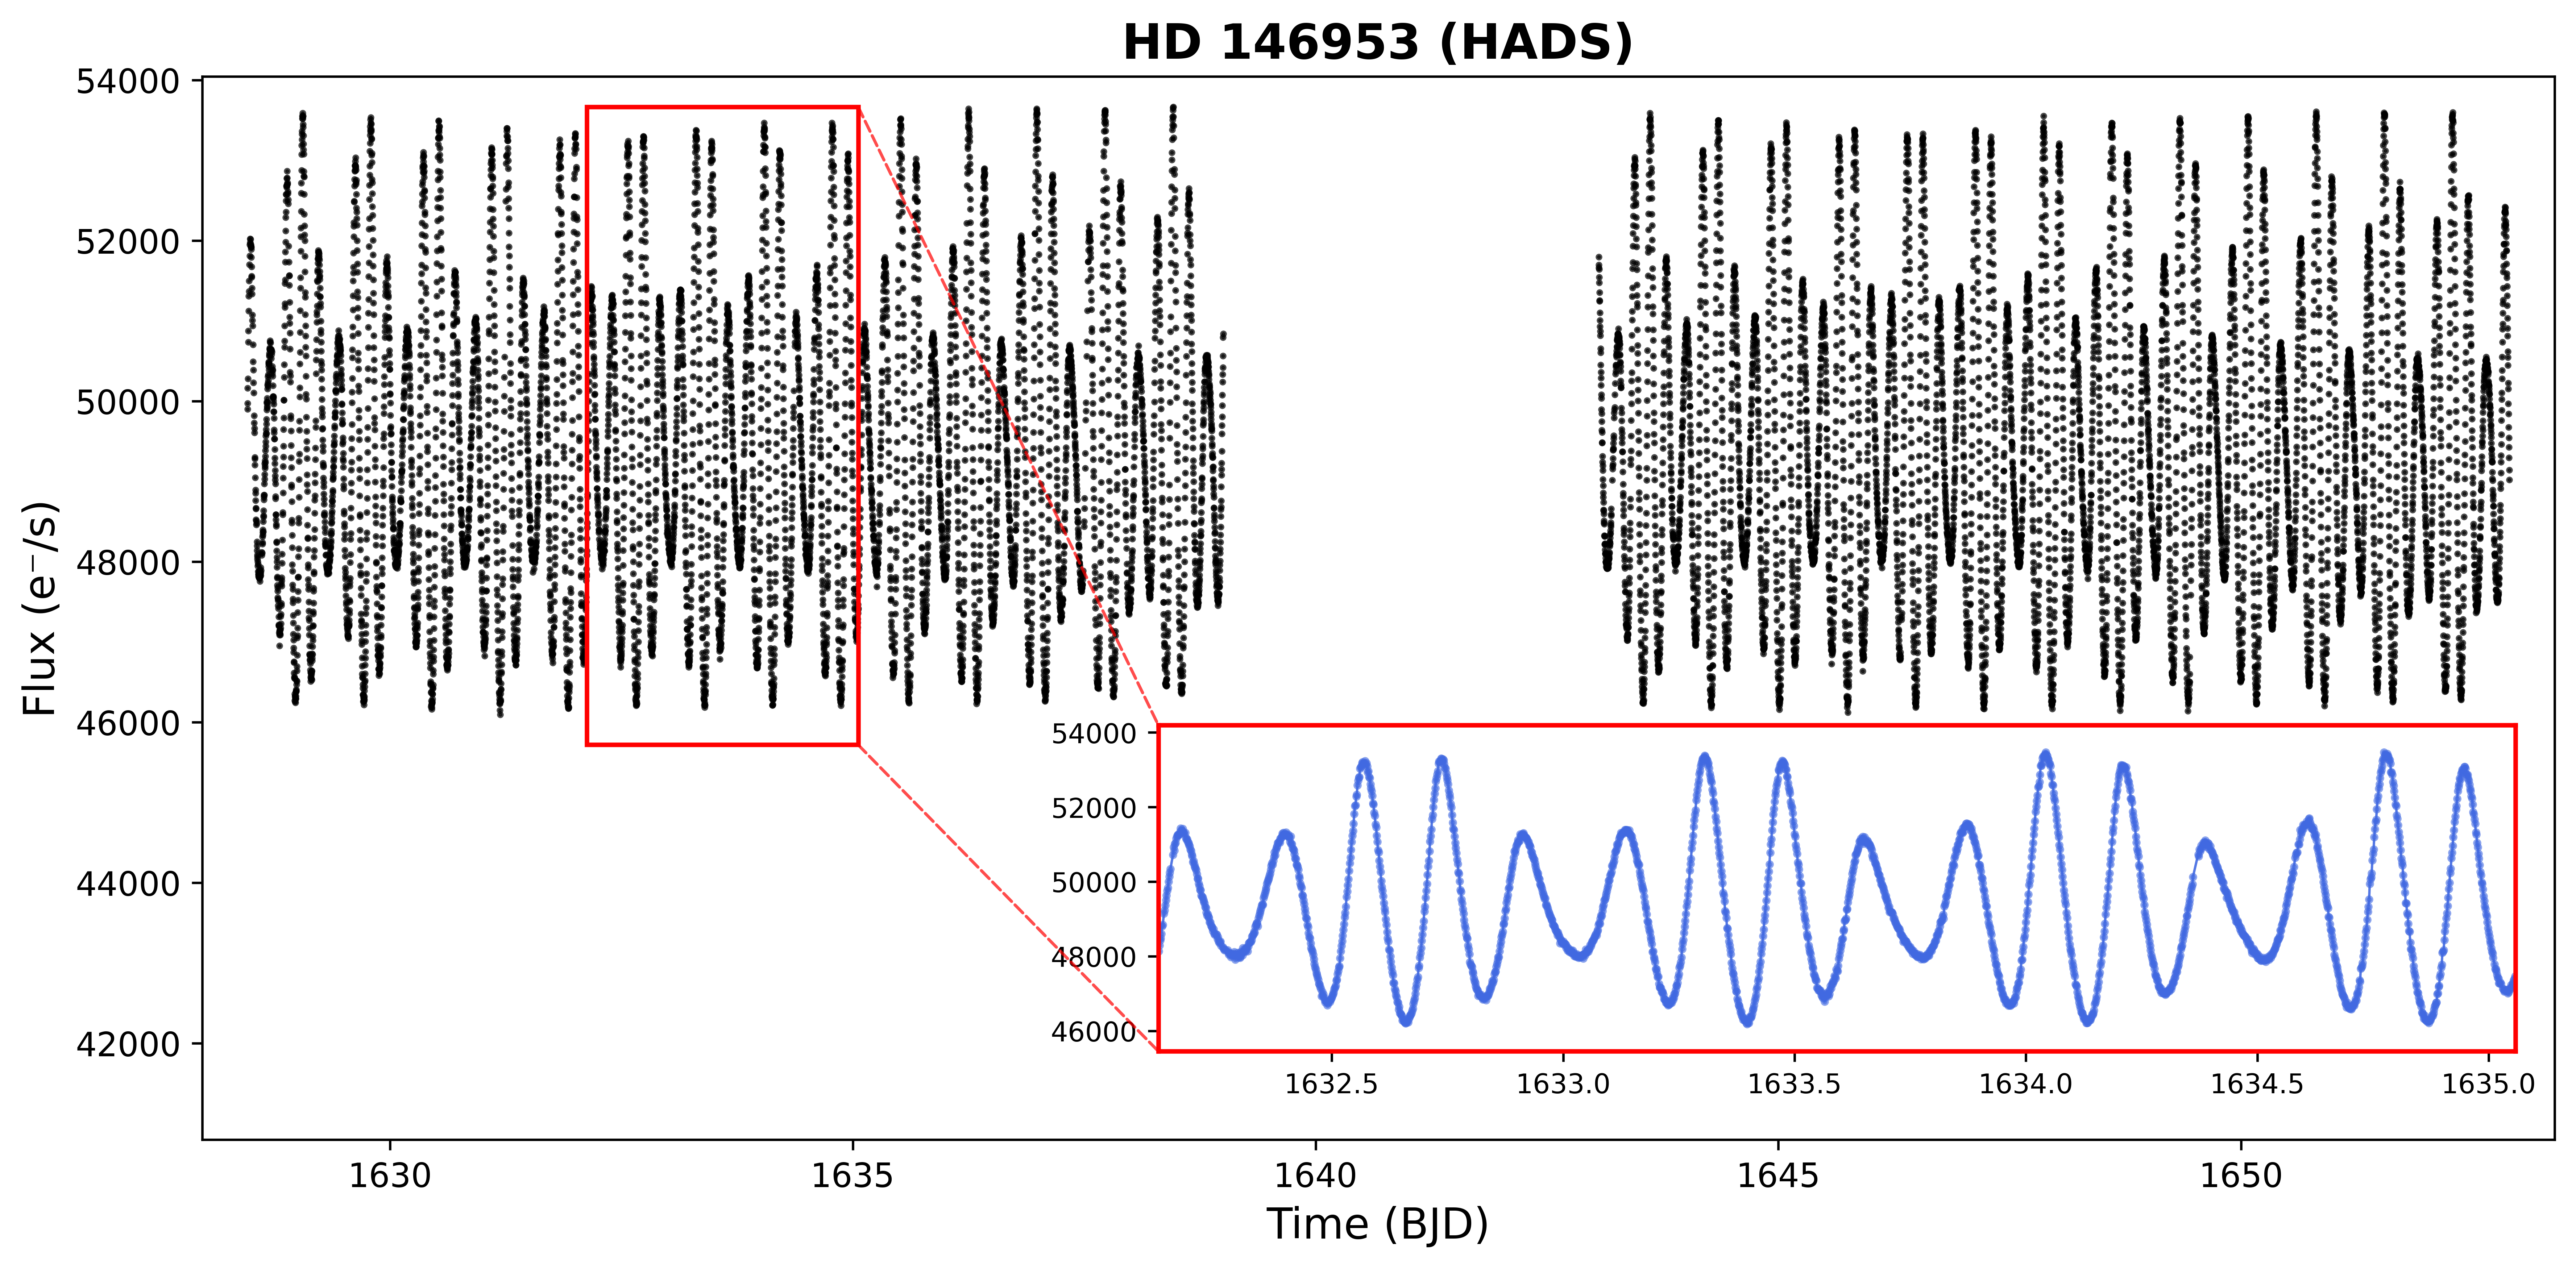
\includegraphics[width=0.6\linewidth]{Images/zoom_plot_HADS_HD_146953.png}
      \caption{Example light curve from the HADS star HD 146953. The inset highlights the regular, high-amplitude oscillation pattern, representing a quasi-stationary signal.}
      \label{fig:hads_example}
    \end{figure}
    
    \item \textbf{LADS:} These stars present multiple superposed frequency components in their flux signal. Consequently, these signals are non-stationary: their statistical properties (specifically, the local variance or amplitude) change throughout the time series (see Figure \ref{fig:lads_example}).
    
    \begin{figure}
      \centering
      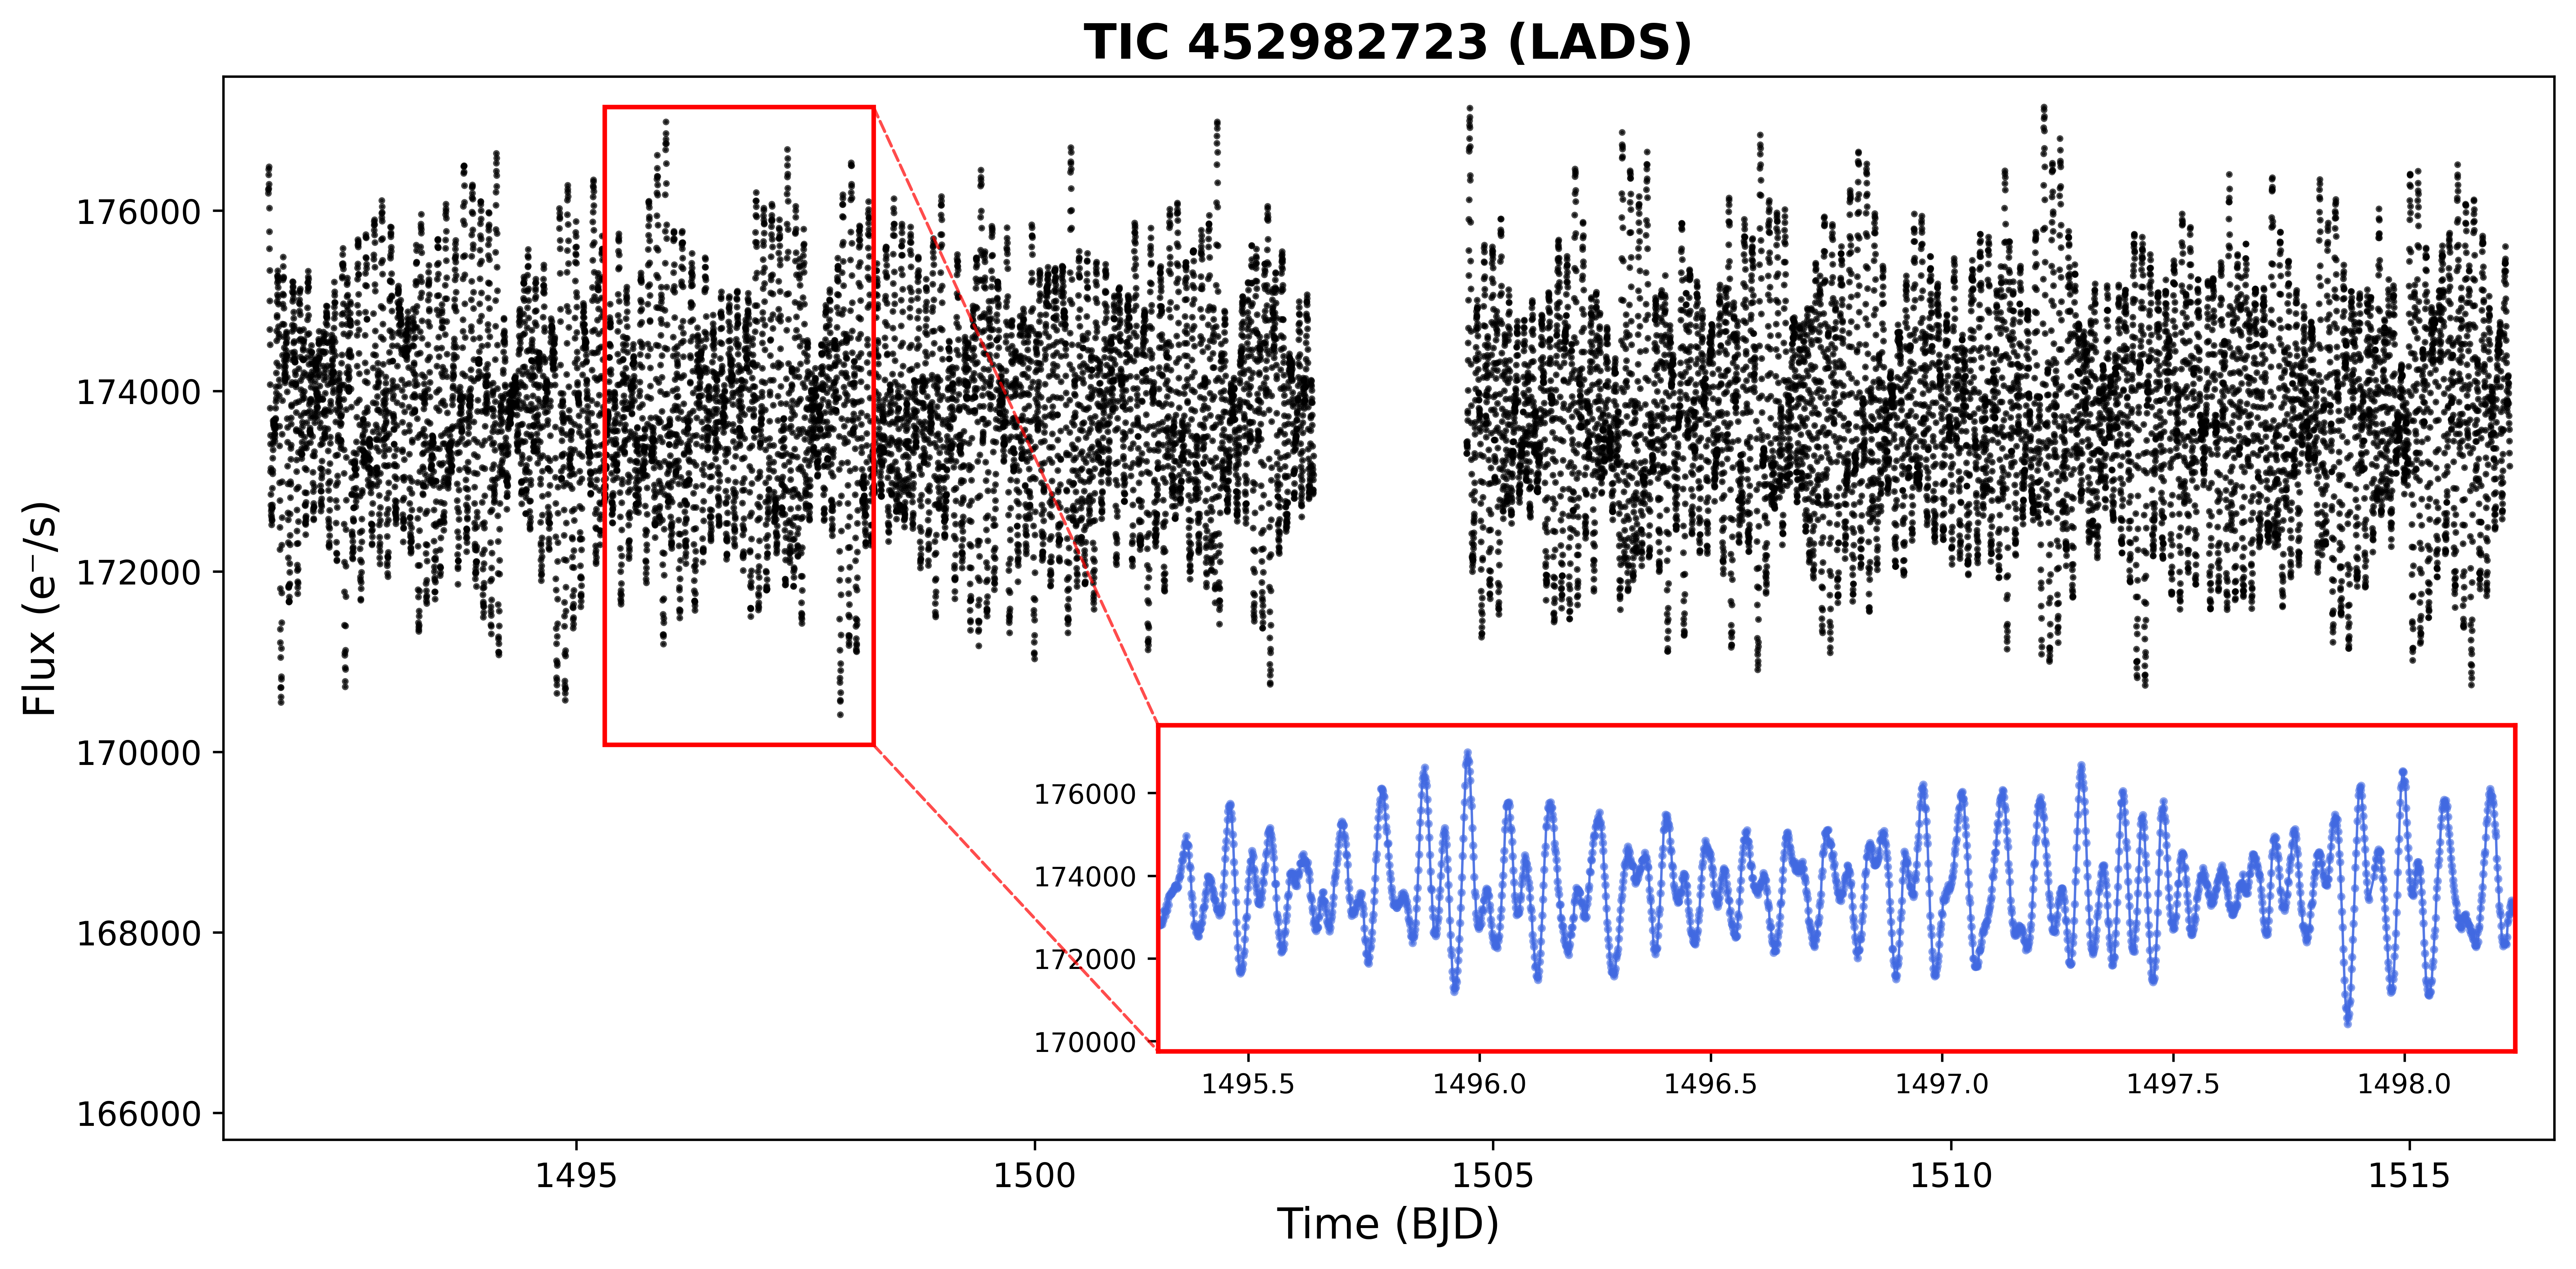
\includegraphics[width=0.6\linewidth]{Images/zoom_plot_LADS_TIC_452982723.png}
      \caption{Example light curve from the LADS star TIC 452982723. The inset reveals the complex multi-frequency oscillations and time-varying amplitude of this non-stationary signal.}
      \label{fig:lads_example}
    \end{figure}

\end{itemize}

The main difficulty lies in the LADS stars. Standard missing data imputation models often assume stationarity, specifically constant amplitude. An effective imputation algorithm must capture not only the rapid periodic oscillations but also their time-varying amplitude to ensure the reconstructed signal matches the global dynamics of the star across large gaps.

\subsection{Algorithms}

 We selected five baselines representing the primary approaches for modeling periodic time series, all configured with frequency information from the Lomb-Scargle periodogram. \textbf{ARMAX} \cite{hyndman2018forecasting} was chosen to represent static harmonic regression models that assume constant amplitude. We included \textbf{GP-Celerite} \cite{foreman2017fast} to represent probabilistic GPs, a non-parametric Bayesian modeling approach, where the dominant Lomb-Scargle frequency is used to initialize the SHOTerm kernel period. For GP-Celerite, we use the \textit{celerite2} library\footnote{\url{https://pypi.org/project/celerite2/}} with a Stochastically-driven Harmonic Oscillator (SHOTerm) kernel to evaluate if non-parametric inference can handle large gaps better than parametric methods. Finally, to evaluate recursive state-space approaches that allow for time-varying amplitudes, we selected \textbf{DHR} \cite{young1999dynamic}, \textbf{TBATS} \cite{de2011forecasting}, and \textbf{FS-BSM} \cite{hindrayanto2013modelling}, which employ distinct tracking mechanisms based on Kalman filtering, exponential smoothing, and frequency-specific disturbance variances, respectively.



\subsection{Experimental Set-up}

We implemented all experiments in Python 3.14 and executed them on a single CPU core of an Intel Core i7-10700K processor at 3.80 GHz. Under this setup, we evaluated performance using 5-fold Cross-Validation (CV). In each fold, we masked a single contiguous gap, evaluating separately gap sizes of $N=1000$ and $N=2000$ data points, using the original flux values as ground truth. We selected these durations to consider the operational range of Delta Scuti stars in TESS. Typical contiguous gaps arise from data downlinks to Earth, which generally interrupt observations for 1 to 2 days. At the standard 2-minute short cadence, this translates to an empirical gap range of 720 to 1440 missing cadences. We evaluated two gap lengths: $N=1000$, representing a typical gap within this empirical range, and $N=2000$, representing an extreme scenario that exceeds it \cite{GarciaHernandez2009HD174936, jenkins2021tess}. {\color{blue}This benchmark focuses on a single contiguous missing-data gap per fold to simulate downlink windows, but it does not evaluate fragmented or multi-gap distributions.} To guarantee a fair comparison, all harmonic and state-space methods utilize the same frequency extraction method (the Lomb-Scargle periodogram) to obtain their dominant frequencies ($f_1, \ldots, f_K$), ensuring every method operates under the same periodic prior information \cite{vanderplas2018understanding}. Finally, we performed a grid search over the hyperparameters of each method (see Table~\ref{tab:hyperparameters_compact}), selecting the optimal configuration for each (star, method) pair that maximizes the coefficient of determination ($R^2$). {\color{blue}We recomputed the Lomb-Scargle periodogram and conducted hyperparameter tuning independently within each fold using only the observed cadences ($t_{\text{obs}}, y_{\text{obs}}$), ensuring that no information from the masked test intervals leaked into model training or selection.} The search space of each hyperparameter reflects its physical role: {\color{blue}the number of frequencies ($K$) reflects the computational bounds of each method, where state-space models (DHR, TBATS, FS-BSM) are constrained to $K \le 5$ due to state-space dimensionality and non-linear optimization limits, whereas R-TVF scales efficiently to higher values of $K$ using a single closed-form ridge regression.} The polynomial degree ($d$) controls the smoothness of the time-varying amplitude evolution, and the regularization strength ($\lambda$) prevents the model from diverging within the unobserved gap.




\begin{table}[htbp]
\centering
\caption{Hyperparameter search space for each imputation method.}
\label{tab:hyperparameters_compact}
\resizebox{0.6\columnwidth}{!}{%
\small
\begin{tabular}{@{}lll@{}}
\toprule
\textbf{Method} & \textbf{Hyperparameter} & \textbf{Search Space} \\
\midrule
\textbf{ARMAX}  & AutoRegressive (AR) order $p$                  & $\{1, 3\}$ \\
                & Moving Average (MA) order $q$ & $\{1, 2\}$ \\
                & Num. Frequencies $K$          & $\{10, 30\}$ \\
\addlinespace
\textbf{GP-Celerite} & Damping $\tau$           & $\{10, 50, 100\}$ days \\
                     & Noise $\sigma_n$         & $\{10^{-3}, 10^{-4}\}$ \\
                     & Period $\rho$            & Auto (Lomb-Scargle) \\
\addlinespace
\textbf{DHR} & Num. Frequencies $K$ & $\{3, 5\}$ \\
                               & AR order $p_{\text{ar}}$ & $\{1, 2\}$ \\
\addlinespace
\textbf{TBATS} & Num. Frequencies $K$ & $\{3, 5\}$ \\
                                 & AR order $p_{\text{ar}}$ & $\{0, 1\}$ \\
\addlinespace
\textbf{FS-BSM} & Num. Frequencies $K$ & $\{3, 5\}$ \\
                                  & Max iterations & $\{20, 50\}$ \\
\addlinespace
\textbf{R-TVF}       & Num. Frequencies $K$     & $\{10, 30, 60\}$ \\
                     & Degree $d$               & $\{1, 3\}$ \\
                     & Reg. strength $\lambda$  & $\{0.0, 0.001, 0.01, 0.1\}$ \\
\bottomrule
\end{tabular}
}
\end{table}


We computed the Mean Absolute Error (MAE) and Mean Squared Error (MSE) to quantify the magnitude of the imputation error. MSE penalizes large deviations \cite{hewamalage2023forecast}. We used the Mean Absolute Percentage Error (MAPE) to provide a scale-independent measure of accuracy. Finally, we employed the Coefficient of Determination ($R^2$) to assess both local accuracy and global variability. To evaluate computational efficiency, we decompose each method's execution time into two phases {\color{blue}for a single run (excluding the hyperparameter grid search)}: Lomb-Scargle Periodogram extraction (LS) and final model fitting (Fit). Although all methods apply the same Lomb-Scargle periodogram estimation, each executes it independently per fold; this decomposition therefore isolates whether any execution time difference arises from frequency extraction or from the model fitting itself. {\color{blue}To support visual assessment of imputation reliability, we display the analytical $3\sigma$ uncertainty band defined in Eq.~(\ref{eq:uncertainty}) in the imputation figures (Figures~\ref{fig:grid_hads} and \ref{fig:robustness_lads_grid}).}




\section{Results} \label{sec:results_discuss}


\subsection{Comparative Performance Analysis for Gaps of $N=1000$} \label{sec:comparative_results}

This section presents the performance evaluation of the proposed R-TVF method compared to five state-of-the-art methods (ARMAX, GP-Celerite, DHR, TBATS, and FS-BSM) for gaps of $N=1000$. Tables \ref{tab:cv_hads} and \ref{tab:cv_lads} summarize the results.

\begin{table*}[htbp]
\centering
\caption{Cross-validation results for HADS stars ($N=1000$). The computational time is decomposed into Lomb-Scargle Periodogram estimation (LS) and final Model Fit (Fit).}
\label{tab:cv_hads}
\resizebox{0.95\textwidth}{!}{%
\begin{tabular}{lcccccc}
\toprule
\textbf{Method} & \textbf{MAE} & \textbf{MSE ($\times 10^6$)} & \textbf{MAPE (\%)} & \textbf{$R^2$} & \textbf{Total Time (s)} & \textbf{LS / Fit (s)} \\
\midrule
ARMAX & \textbf{1386 $\pm$ 3467} & \textbf{20.9 $\pm$ 100.9} & 151.3 $\pm$ 97.3 & 0.947 $\pm$ 0.045 & 56.2 $\pm$ 33.9 & 0.04 / 56.16 \\
GP-Celerite & 3511 $\pm$ 7870 & 113.4 $\pm$ 475.4 & 485.4 $\pm$ 368.3 & 0.375 $\pm$ 0.617 & \textbf{0.52 $\pm$ 0.12} & 0.04 / 0.48 \\
DHR & 4510 $\pm$ 2145 & 145.2 $\pm$ 82.5 & 450.5 $\pm$ 215.3 & 0.206 $\pm$ 0.229 & 15.3 $\pm$ 4.2 & 0.04 / 15.26 \\
TBATS & 3150 $\pm$ 1500 & 95.6 $\pm$ 40.2 & 380.4 $\pm$ 120.5 & 0.452 $\pm$ 0.154 & 18.5 $\pm$ 5.1 & 0.05 / 18.45 \\
FS-BSM & 1693 $\pm$ 1250 & 59.4 $\pm$ 45.2 & 169.9 $\pm$ 60.5 & 0.928 $\pm$ 0.062 & 24.8 $\pm$ 8.5 & 0.05 / 24.75 \\
R-TVF (ours) & 1429 $\pm$ 6459 & 60.2 $\pm$ 348.8 & \textbf{56.3 $\pm$ 58.2} & \textbf{0.987 $\pm$ 0.045} & 10.6 $\pm$ 3.5 & 0.06 / 10.54 \\
\bottomrule
\end{tabular}%
}
\end{table*}




\begin{table*}[htbp]
\centering
\caption{Cross-validation results for LADS stars ($N=1000$). The computational time is decomposed into Lomb-Scargle Periodogram estimation (LS) and final Model Fit (Fit).}
\label{tab:cv_lads}
\resizebox{0.95\textwidth}{!}{%
\begin{tabular}{lcccccc}
\toprule
\textbf{Method} & \textbf{MAE} & \textbf{MSE ($\times 10^3$)} & \textbf{MAPE (\%)} & \textbf{$R^2$} & \textbf{Total Time (s)} & \textbf{LS / Fit (s)} \\
\midrule
ARMAX & 191 $\pm$ 279 & 173.8 $\pm$ 533.8 & 17.3 $\pm$ 18.6 & 0.791 $\pm$ 0.110 & 77.7 $\pm$ 44.5 & 0.04 / 77.66 \\
GP-Celerite & 647 $\pm$ 942 & 1856.5 $\pm$ 5851.6 & 64.5 $\pm$ 84.3 & -2.873 $\pm$ 6.647 & \textbf{0.59 $\pm$ 0.13} & 0.03 / 0.56 \\
DHR & 420 $\pm$ 250 & 950.4 $\pm$ 450.2 & 35.4 $\pm$ 25.1 & 0.158 $\pm$ 0.420 & 17.4 $\pm$ 5.2 & 0.04 / 17.36 \\
TBATS & 435 $\pm$ 260 & 985.6 $\pm$ 480.5 & 38.2 $\pm$ 28.4 & 0.152 $\pm$ 0.198 & 19.1 $\pm$ 6.3 & 0.04 / 19.06 \\
FS-BSM & 220 $\pm$ 150 & 280.5 $\pm$ 180.2 & 20.0 $\pm$ 15.5 & 0.639 $\pm$ 0.190 & 25.2 $\pm$ 9.1 & 0.06 / 25.14 \\
R-TVF (ours) & \textbf{170 $\pm$ 249} & \textbf{139.1 $\pm$ 428.7} & \textbf{13.9 $\pm$ 11.2} & \textbf{0.816 $\pm$ 0.128} & 9.6 $\pm$ 1.6 & 0.04 / 9.56 \\
\bottomrule
\end{tabular}%
}
\end{table*}

Regarding the HADS stars (Table \ref{tab:cv_hads}), the proposed R-TVF algorithm achieved the highest coefficient of determination ($R^2 = 0.987 \pm 0.045$) and the lowest relative error (MAPE $= 56.3 \pm 58.2\%$). ARMAX was the second-best performing method with an $R^2$ of $0.947 \pm 0.045$, recording the lowest absolute error metrics (MAE $= 1386 \pm 3467$ and MSE $= 20.9 \times 10^6 \pm 100.9 \times 10^6$), followed by FS-BSM with an $R^2$ of $0.928 \pm 0.062$ and MAPE of $169.9 \pm 60.5\%$. TBATS reached an $R^2$ of $0.452 \pm 0.154$. In contrast, GP-Celerite and DHR yielded $R^2$ values below $0.40$ (GP-Celerite: $0.375 \pm 0.617$, DHR: $0.206 \pm 0.229$), with significantly higher error magnitudes. In terms of computational cost, GP-Celerite was the fastest ($0.52$ s), followed by R-TVF ($10.6$ s), DHR ($15.3$ s), TBATS ($18.5$ s), and FS-BSM ($24.8$ s), while ARMAX required the longest computation time ($56.2$ s).

For the LADS stars (Table \ref{tab:cv_lads}), R-TVF obtained the best performance across all accuracy and error metrics. It achieved an $R^2$ of $0.816 \pm 0.128$, an MAE of $170$, and a MAPE of $13.9\%$. ARMAX remained the second-best performing algorithm, with an $R^2$ of $0.791$ and an MAE of $191$. The performance gap widened for the other methods compared to the HADS case: FS-BSM dropped to an $R^2$ of $0.639 \pm 0.190$, while DHR and TBATS recorded $R^2$ values of $0.158 \pm 0.420$ and $0.152 \pm 0.198$, respectively. GP-Celerite recorded a negative mean $R^2$ value ($-2.873 \pm 6.647$), indicating a model that fits worse than a horizontal mean line. Regarding execution time, GP-Celerite was the fastest ($0.59$ s), followed by R-TVF ($9.6$ s), DHR ($17.4$ s), TBATS ($19.1$ s), and FS-BSM ($25.2$ s), while ARMAX was approximately 8 times slower ($77.7$ s) than R-TVF.

To analyze the performance distribution beyond global averages, Figure \ref{fig:swarm_all_stars} displays the individual $R^2$ scores across all folds. R-TVF and ARMAX show tight clustering near $R^2 = 1.0$, indicating consistent performance, whereas the other methods exhibit higher variance with a broader spread of lower scores. Furthermore, Figure \ref{fig:pairwise_scatter} provides a direct pairwise comparison between R-TVF and each baseline. Points lying below the diagonal indicate instances where R-TVF outperforms the other methods. The plot reveals that R-TVF consistently dominates throughout the dataset, particularly against TBATS and DHR, where it achieves higher scores in all individual cases.



\begin{figure}[pos=htbp]
  \centering
  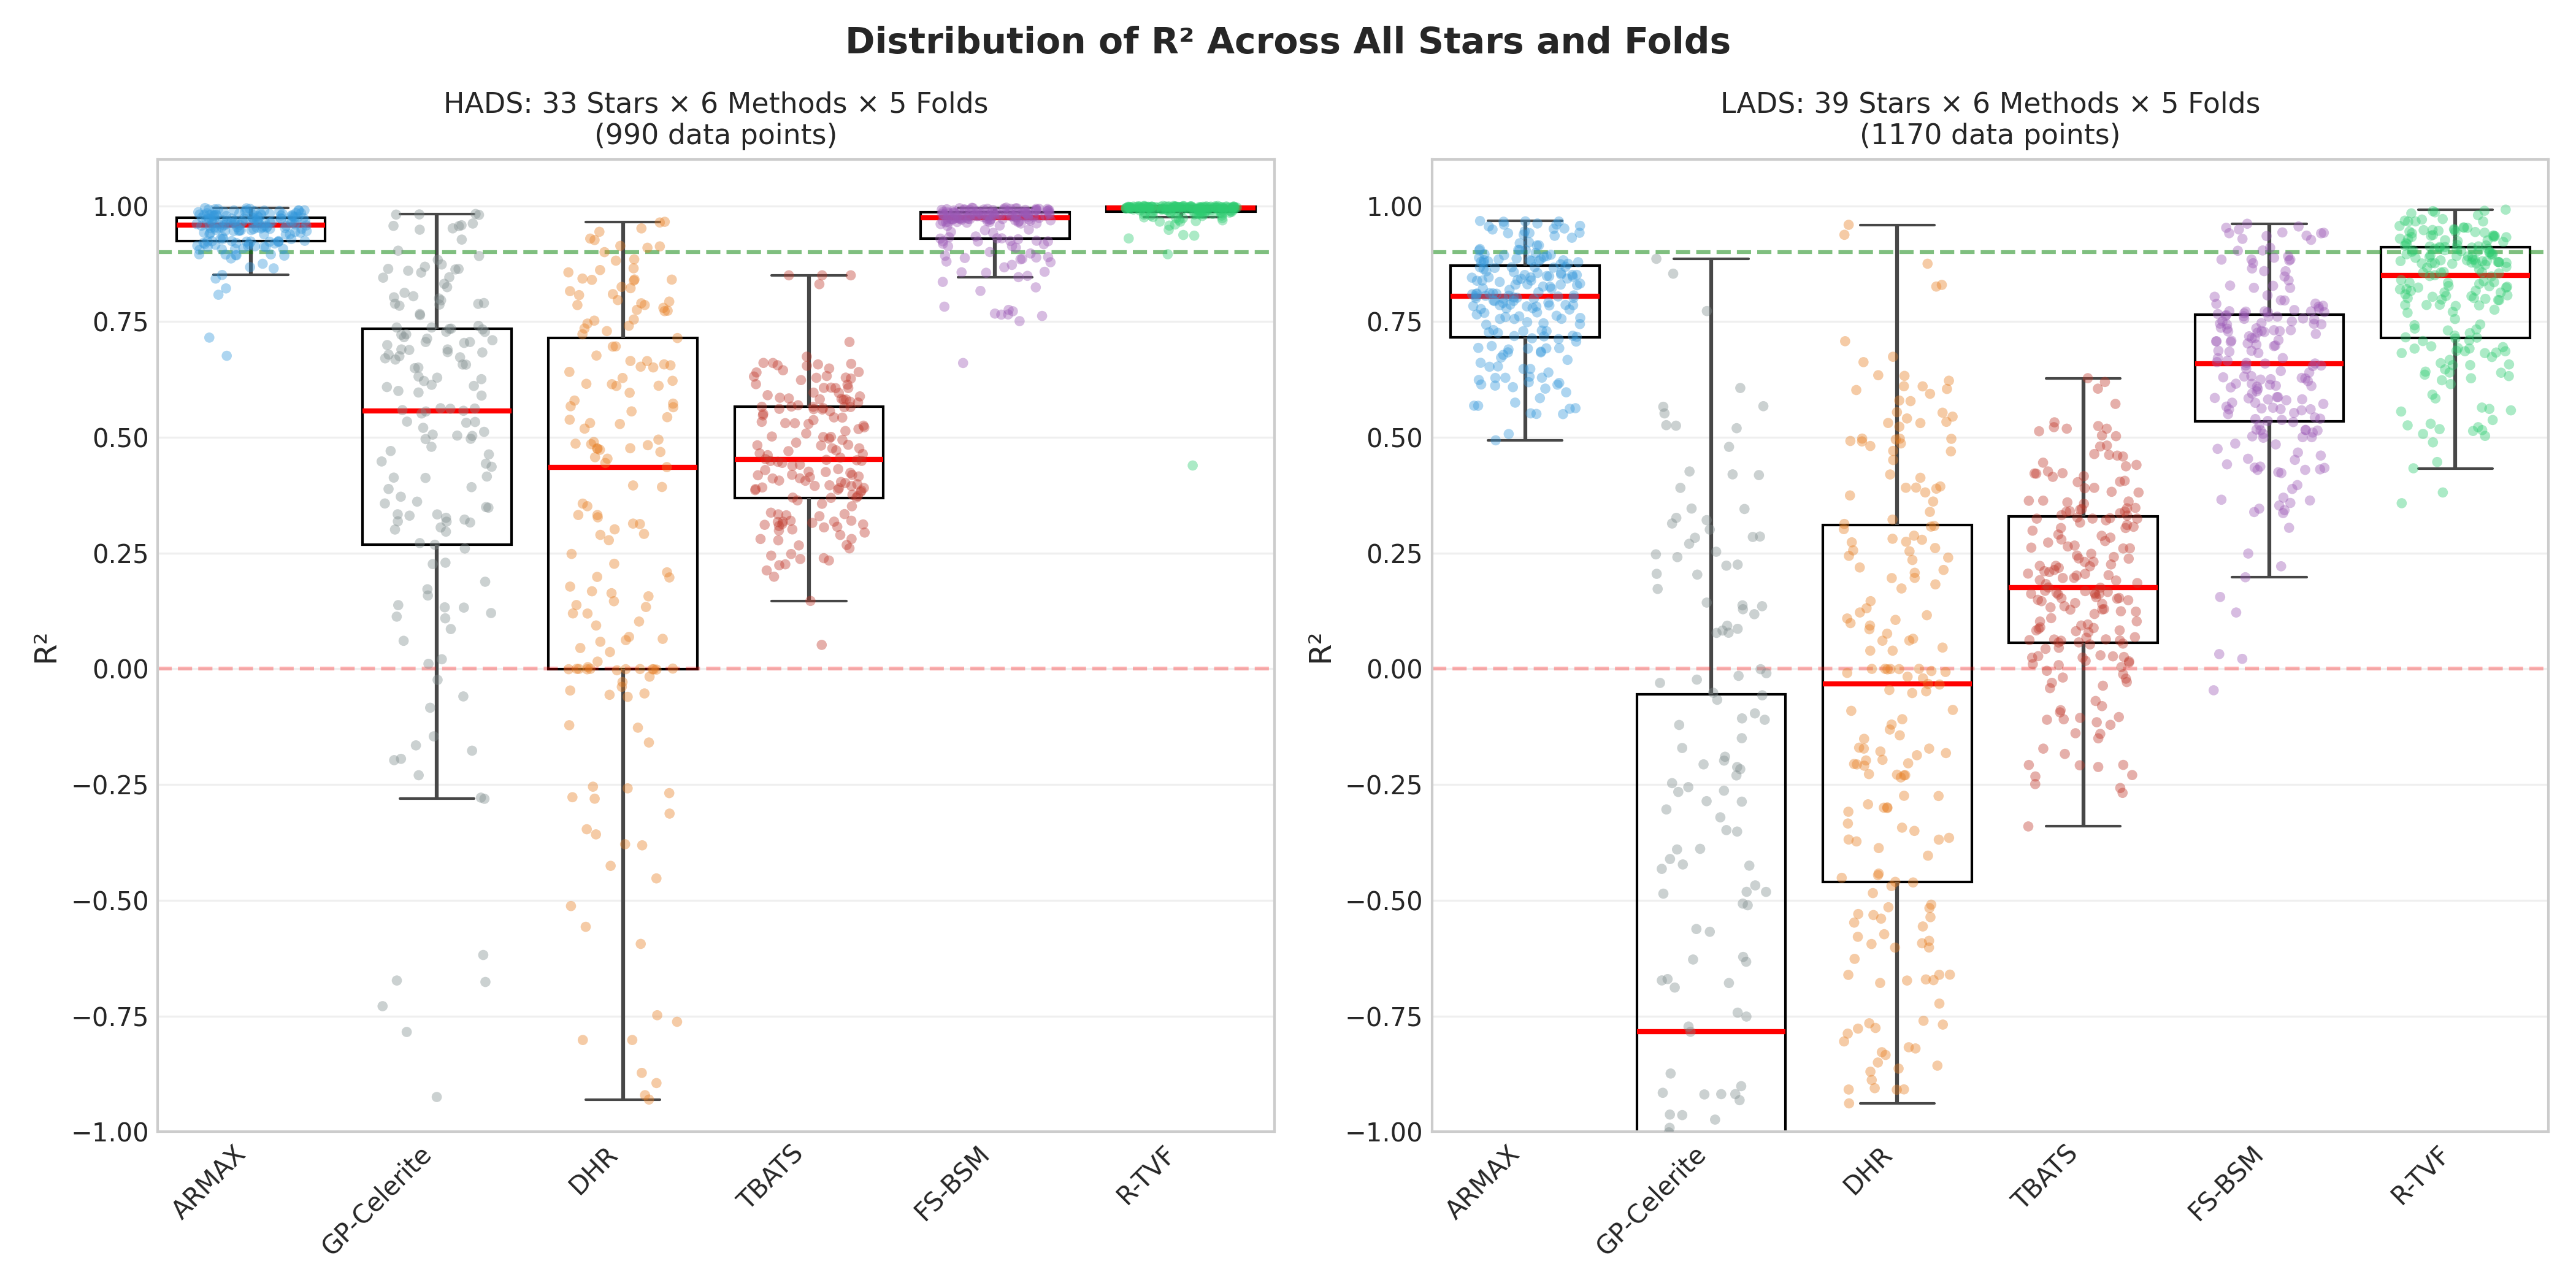
\includegraphics[width=0.9\linewidth]{Images/swarm_all_stars_2nd_sub.png}
  \caption{Distribution of $R^2$ values for each method across all 72 stars and 5 CV folds. Each point represents one (star, fold) evaluation.}
  \label{fig:swarm_all_stars}
\end{figure}


\begin{figure}[pos=htbp]
  \centering
  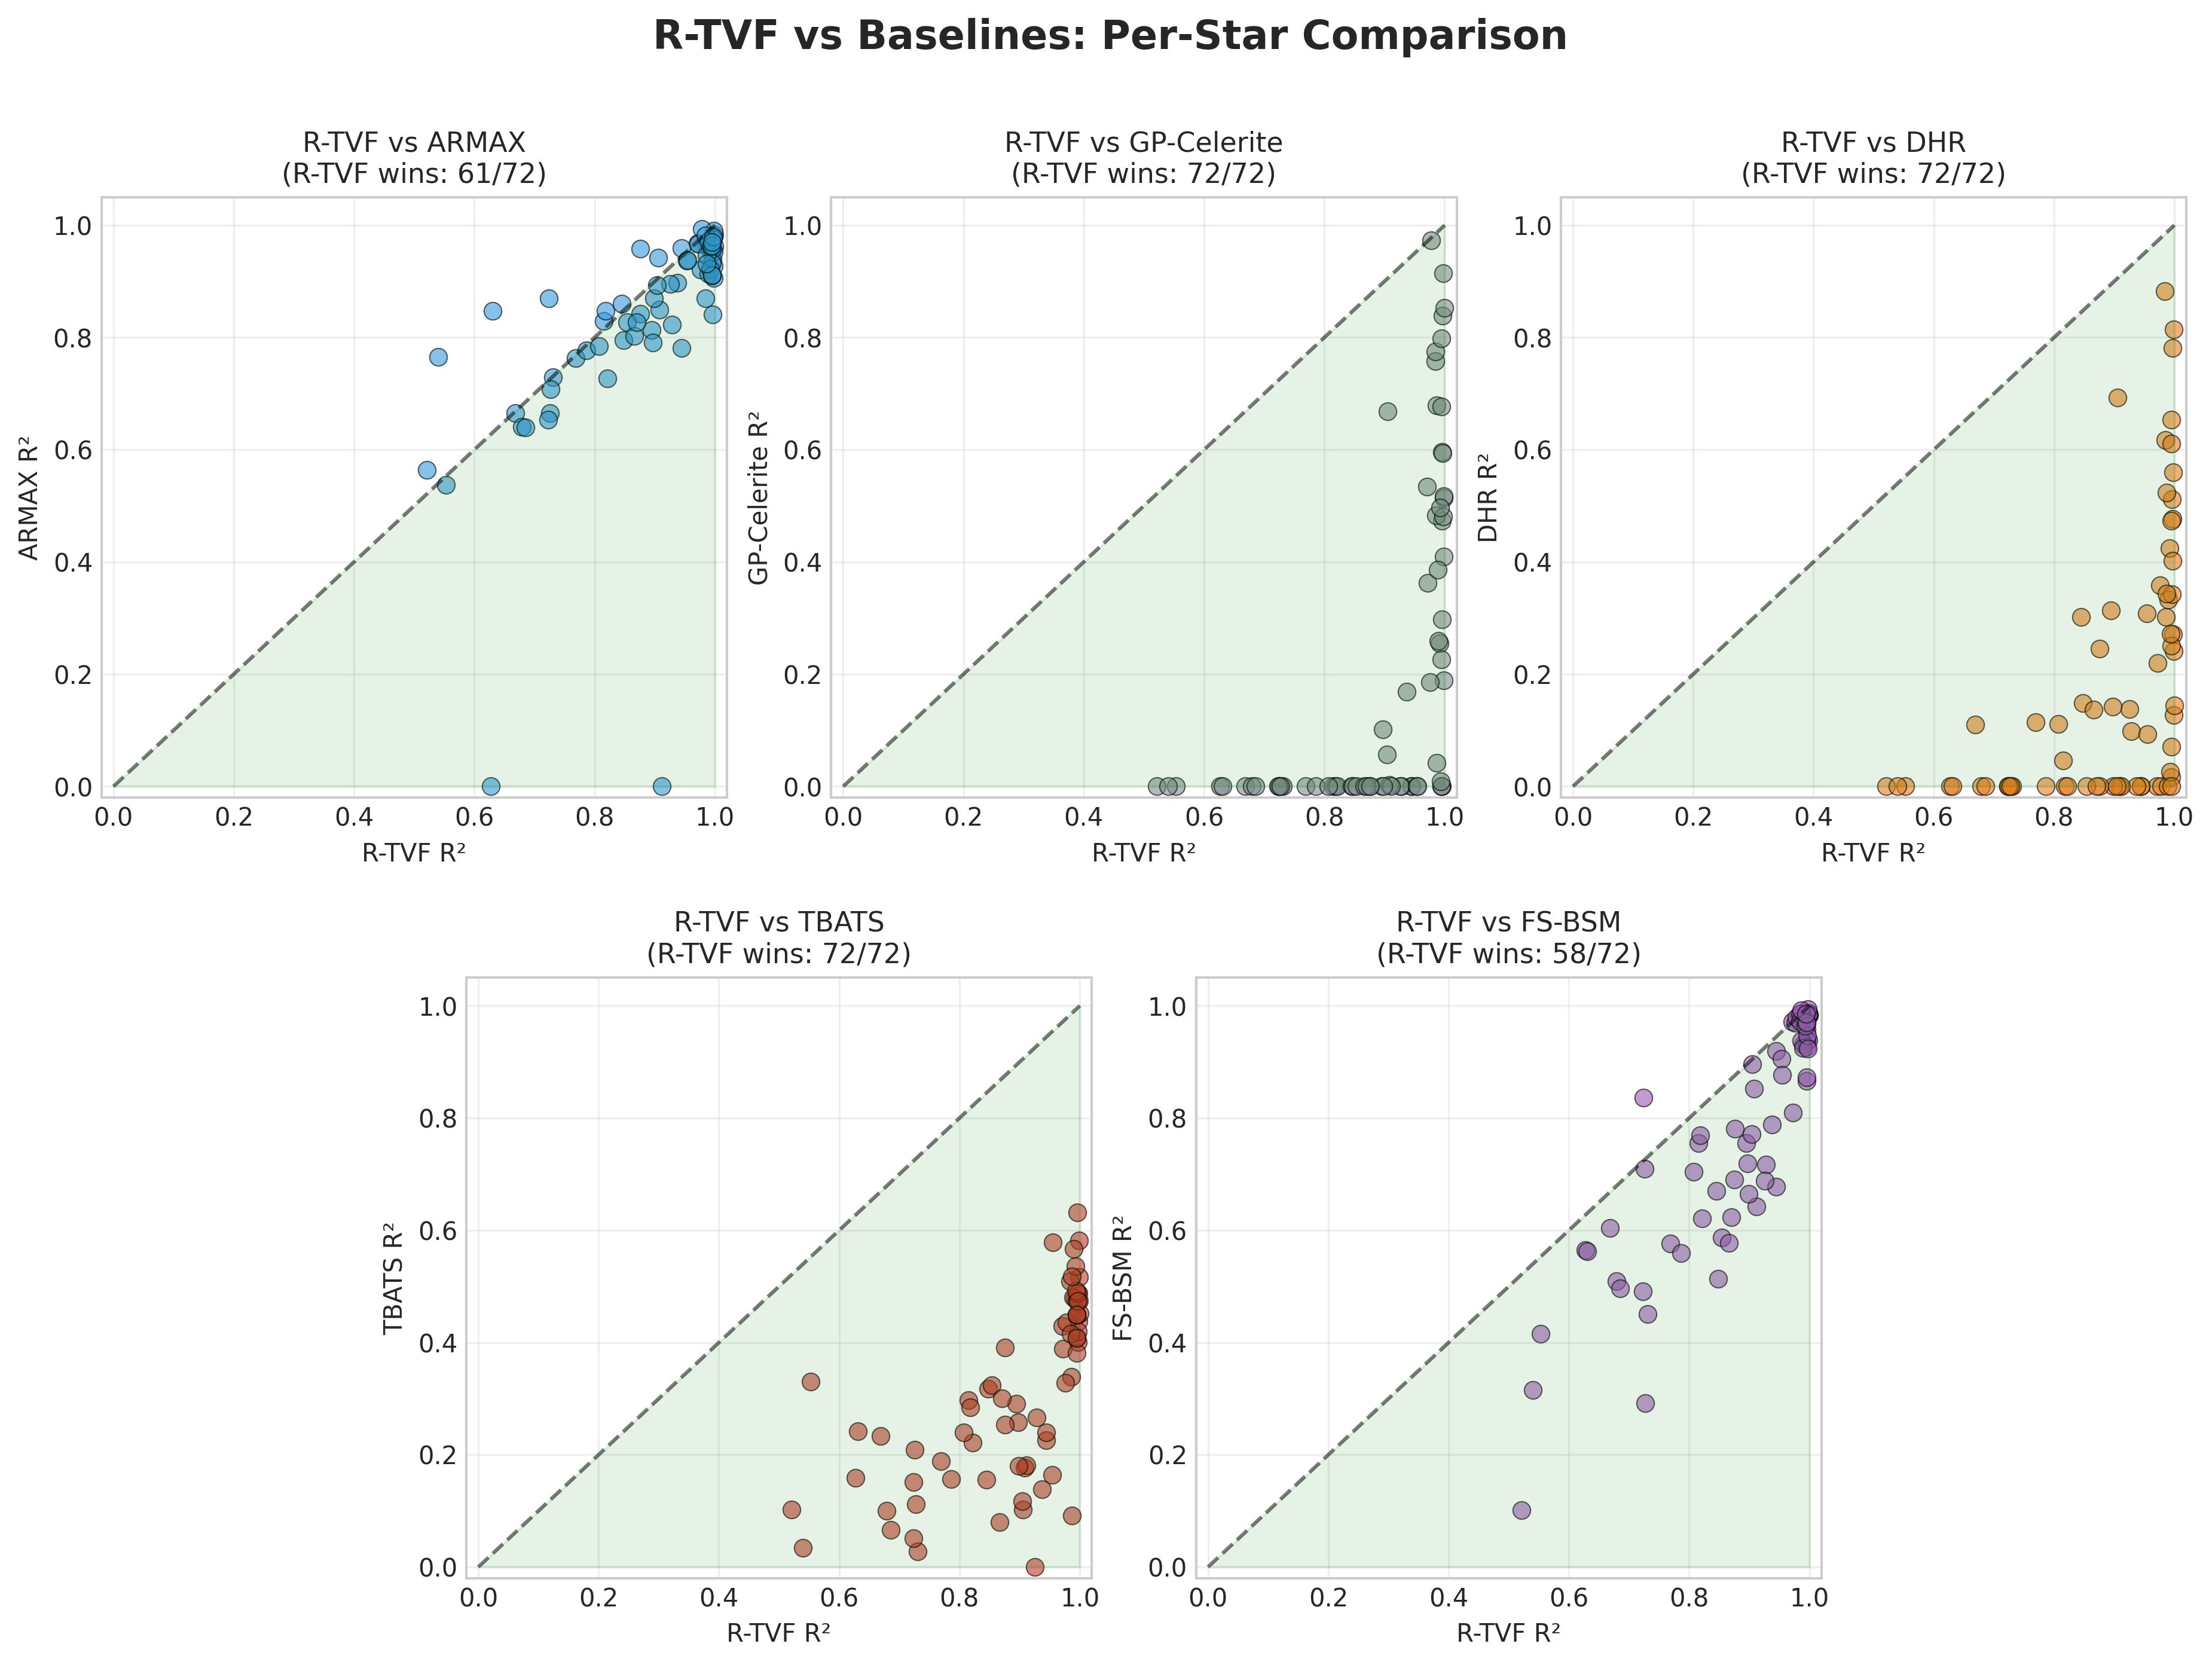
\includegraphics[width=0.9\linewidth]{Images/pairwise_scatter_bounded_2nd_sub.png}
  \caption{Pairwise comparison of $R^2$ between R-TVF and each baseline method. Each point represents one star. Points below the diagonal indicate R-TVF superiority. For visual clarity, negative $R^2$ values (indicating performance worse than the mean) are bounded at 0.}
  \label{fig:pairwise_scatter}
\end{figure}



Finally, to provide visual verification of the imputation quality, Figures \ref{fig:grid_hads} and \ref{fig:grid_lads} present representative imputations for a HADS and a LADS star, respectively. In the HADS star HD 146953 (Fig. \ref{fig:grid_hads}), R-TVF accurately recovers the phase and frequency of the high-amplitude flux signal, whereas competing methods often flatten the signal peaks or introduce phase shifts. For the LADS star TIC 452982723 (Fig. \ref{fig:grid_lads}), R-TVF successfully models the multi-frequency components without the smoothing artifacts observed in harmonic state-space predictions (DHR, TBATS).

\begin{figure}[pos=htbp]
  \centering
  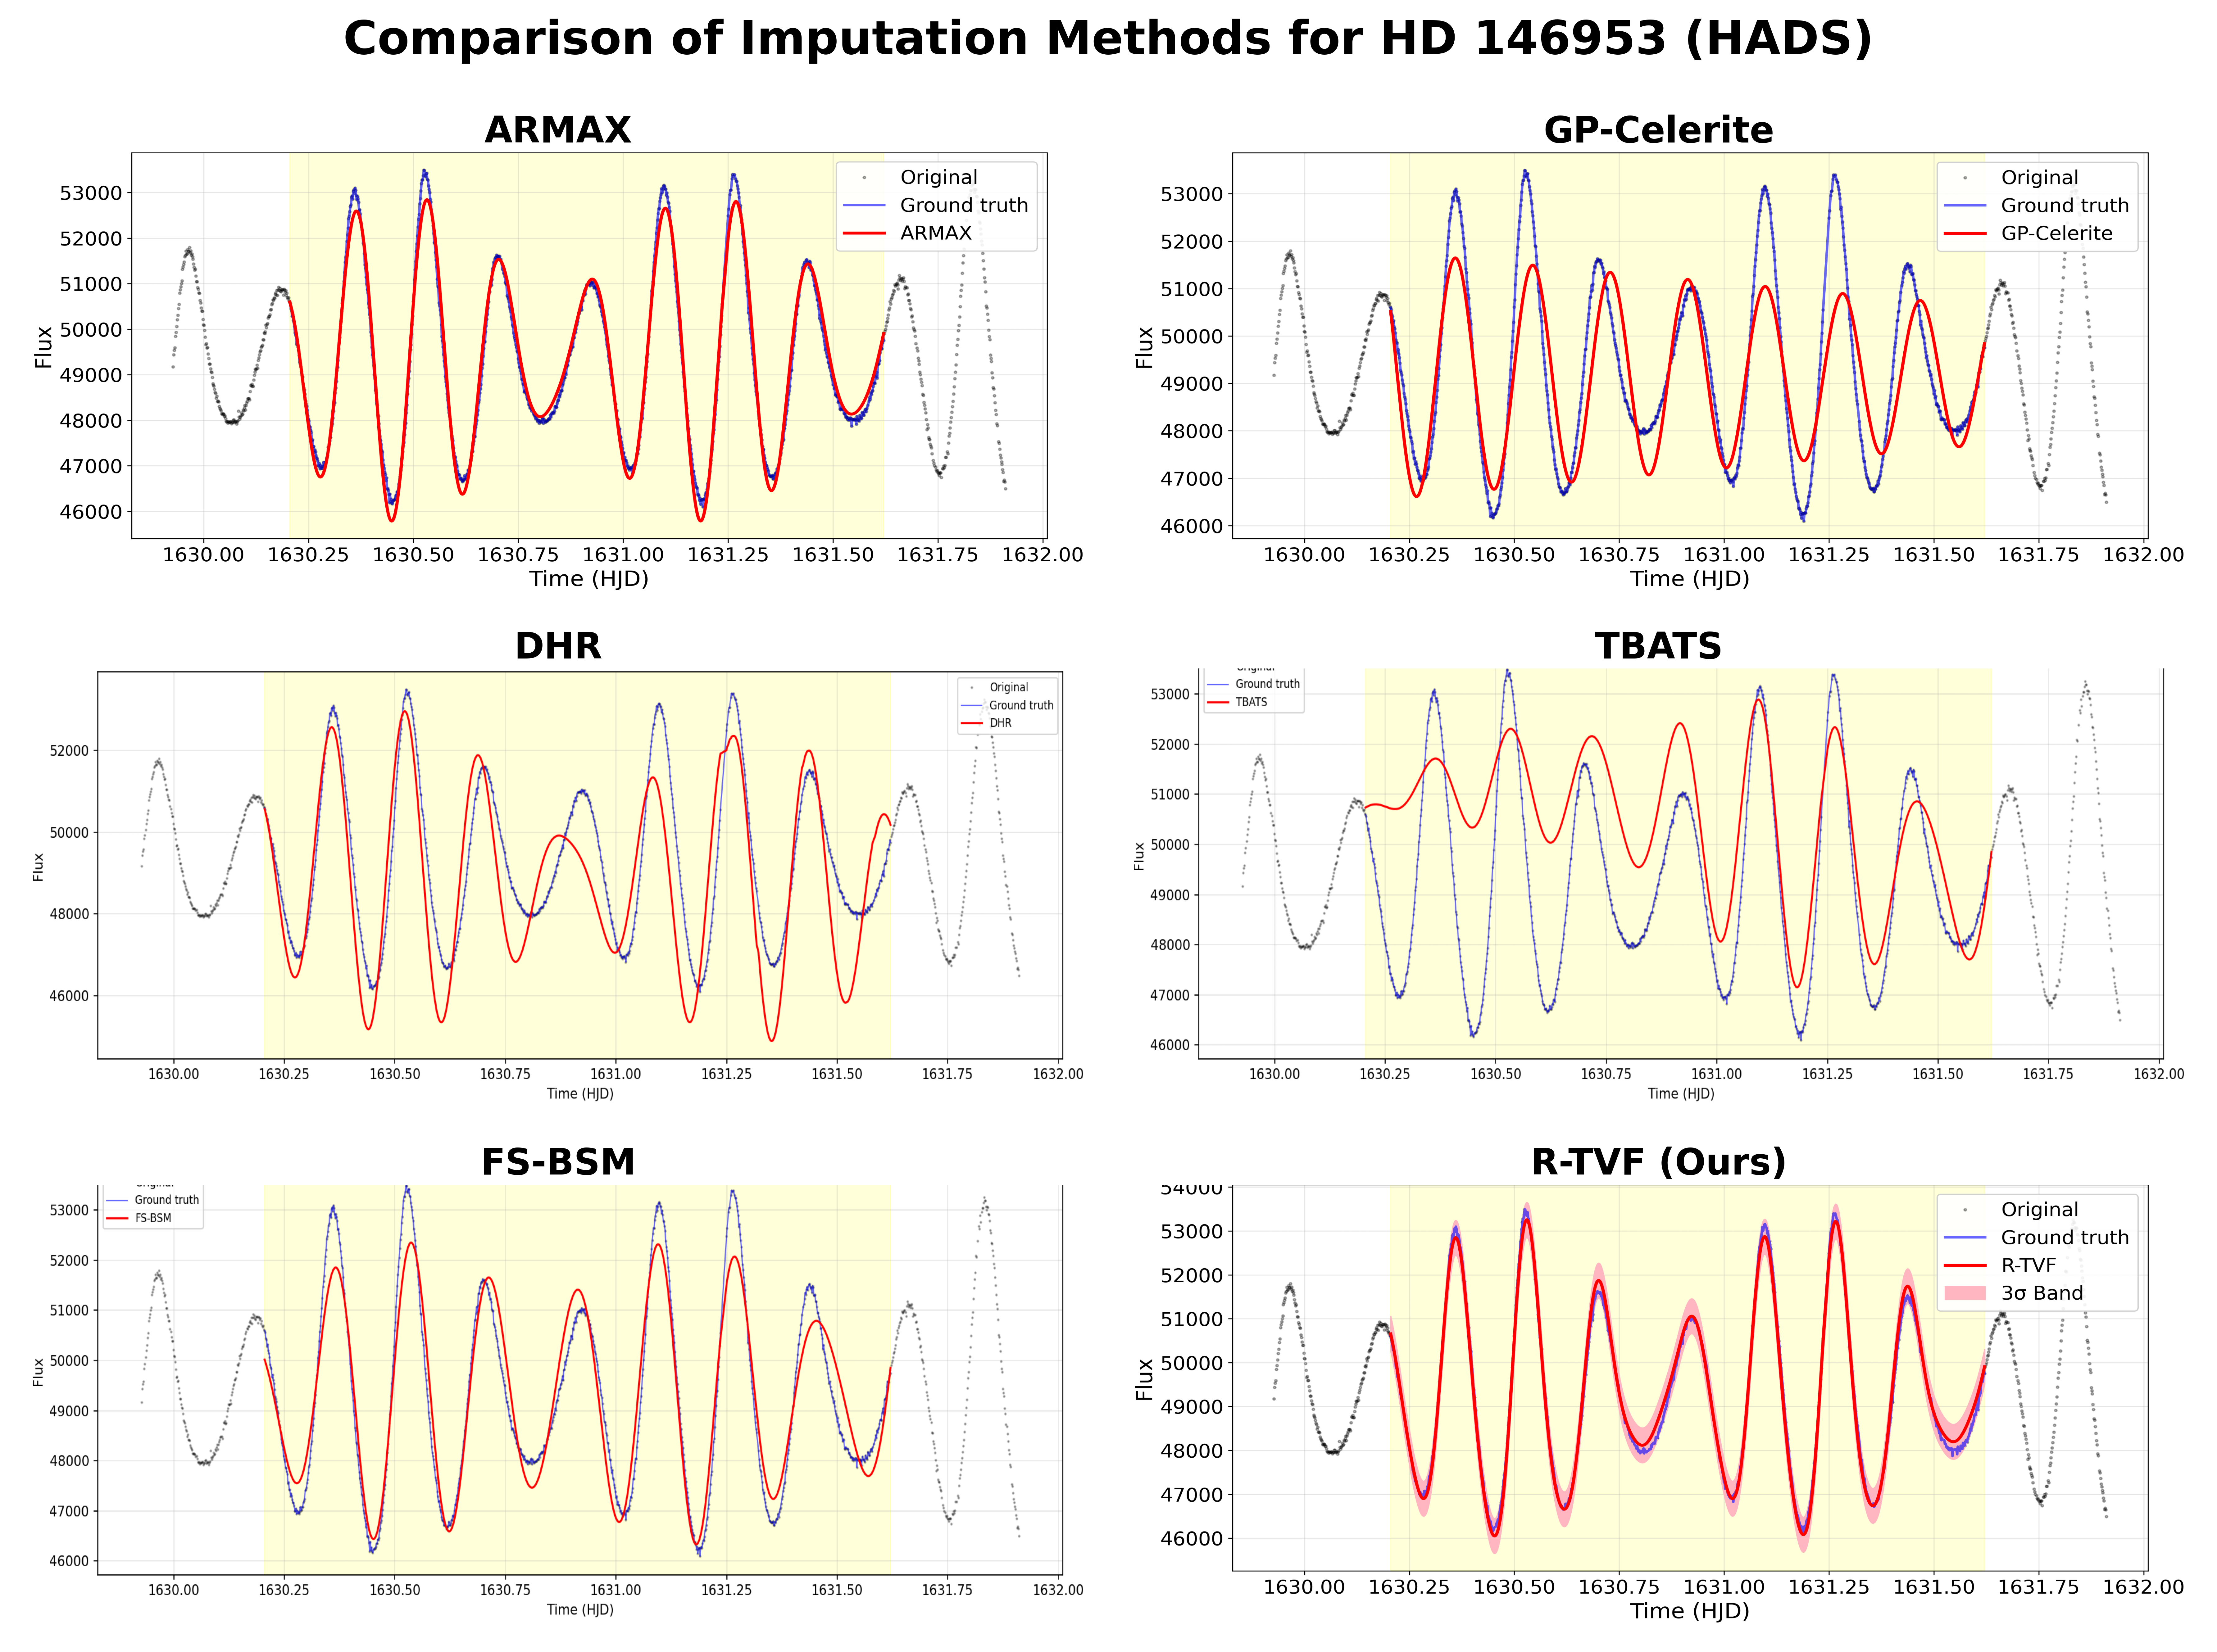
\includegraphics[width=0.9\linewidth]{Images/grid_comparison_HD146953_large.png}
  \caption{Comparison of imputation methods for the HADS star HD 146953. The yellow shaded region indicates the missing data gap (1000 points). The $3\sigma$ analytical uncertainty band (shaded pink) bounds the R-TVF predictions.}
  \label{fig:grid_hads}
\end{figure}


\begin{figure}[pos=htbp]
  \centering
  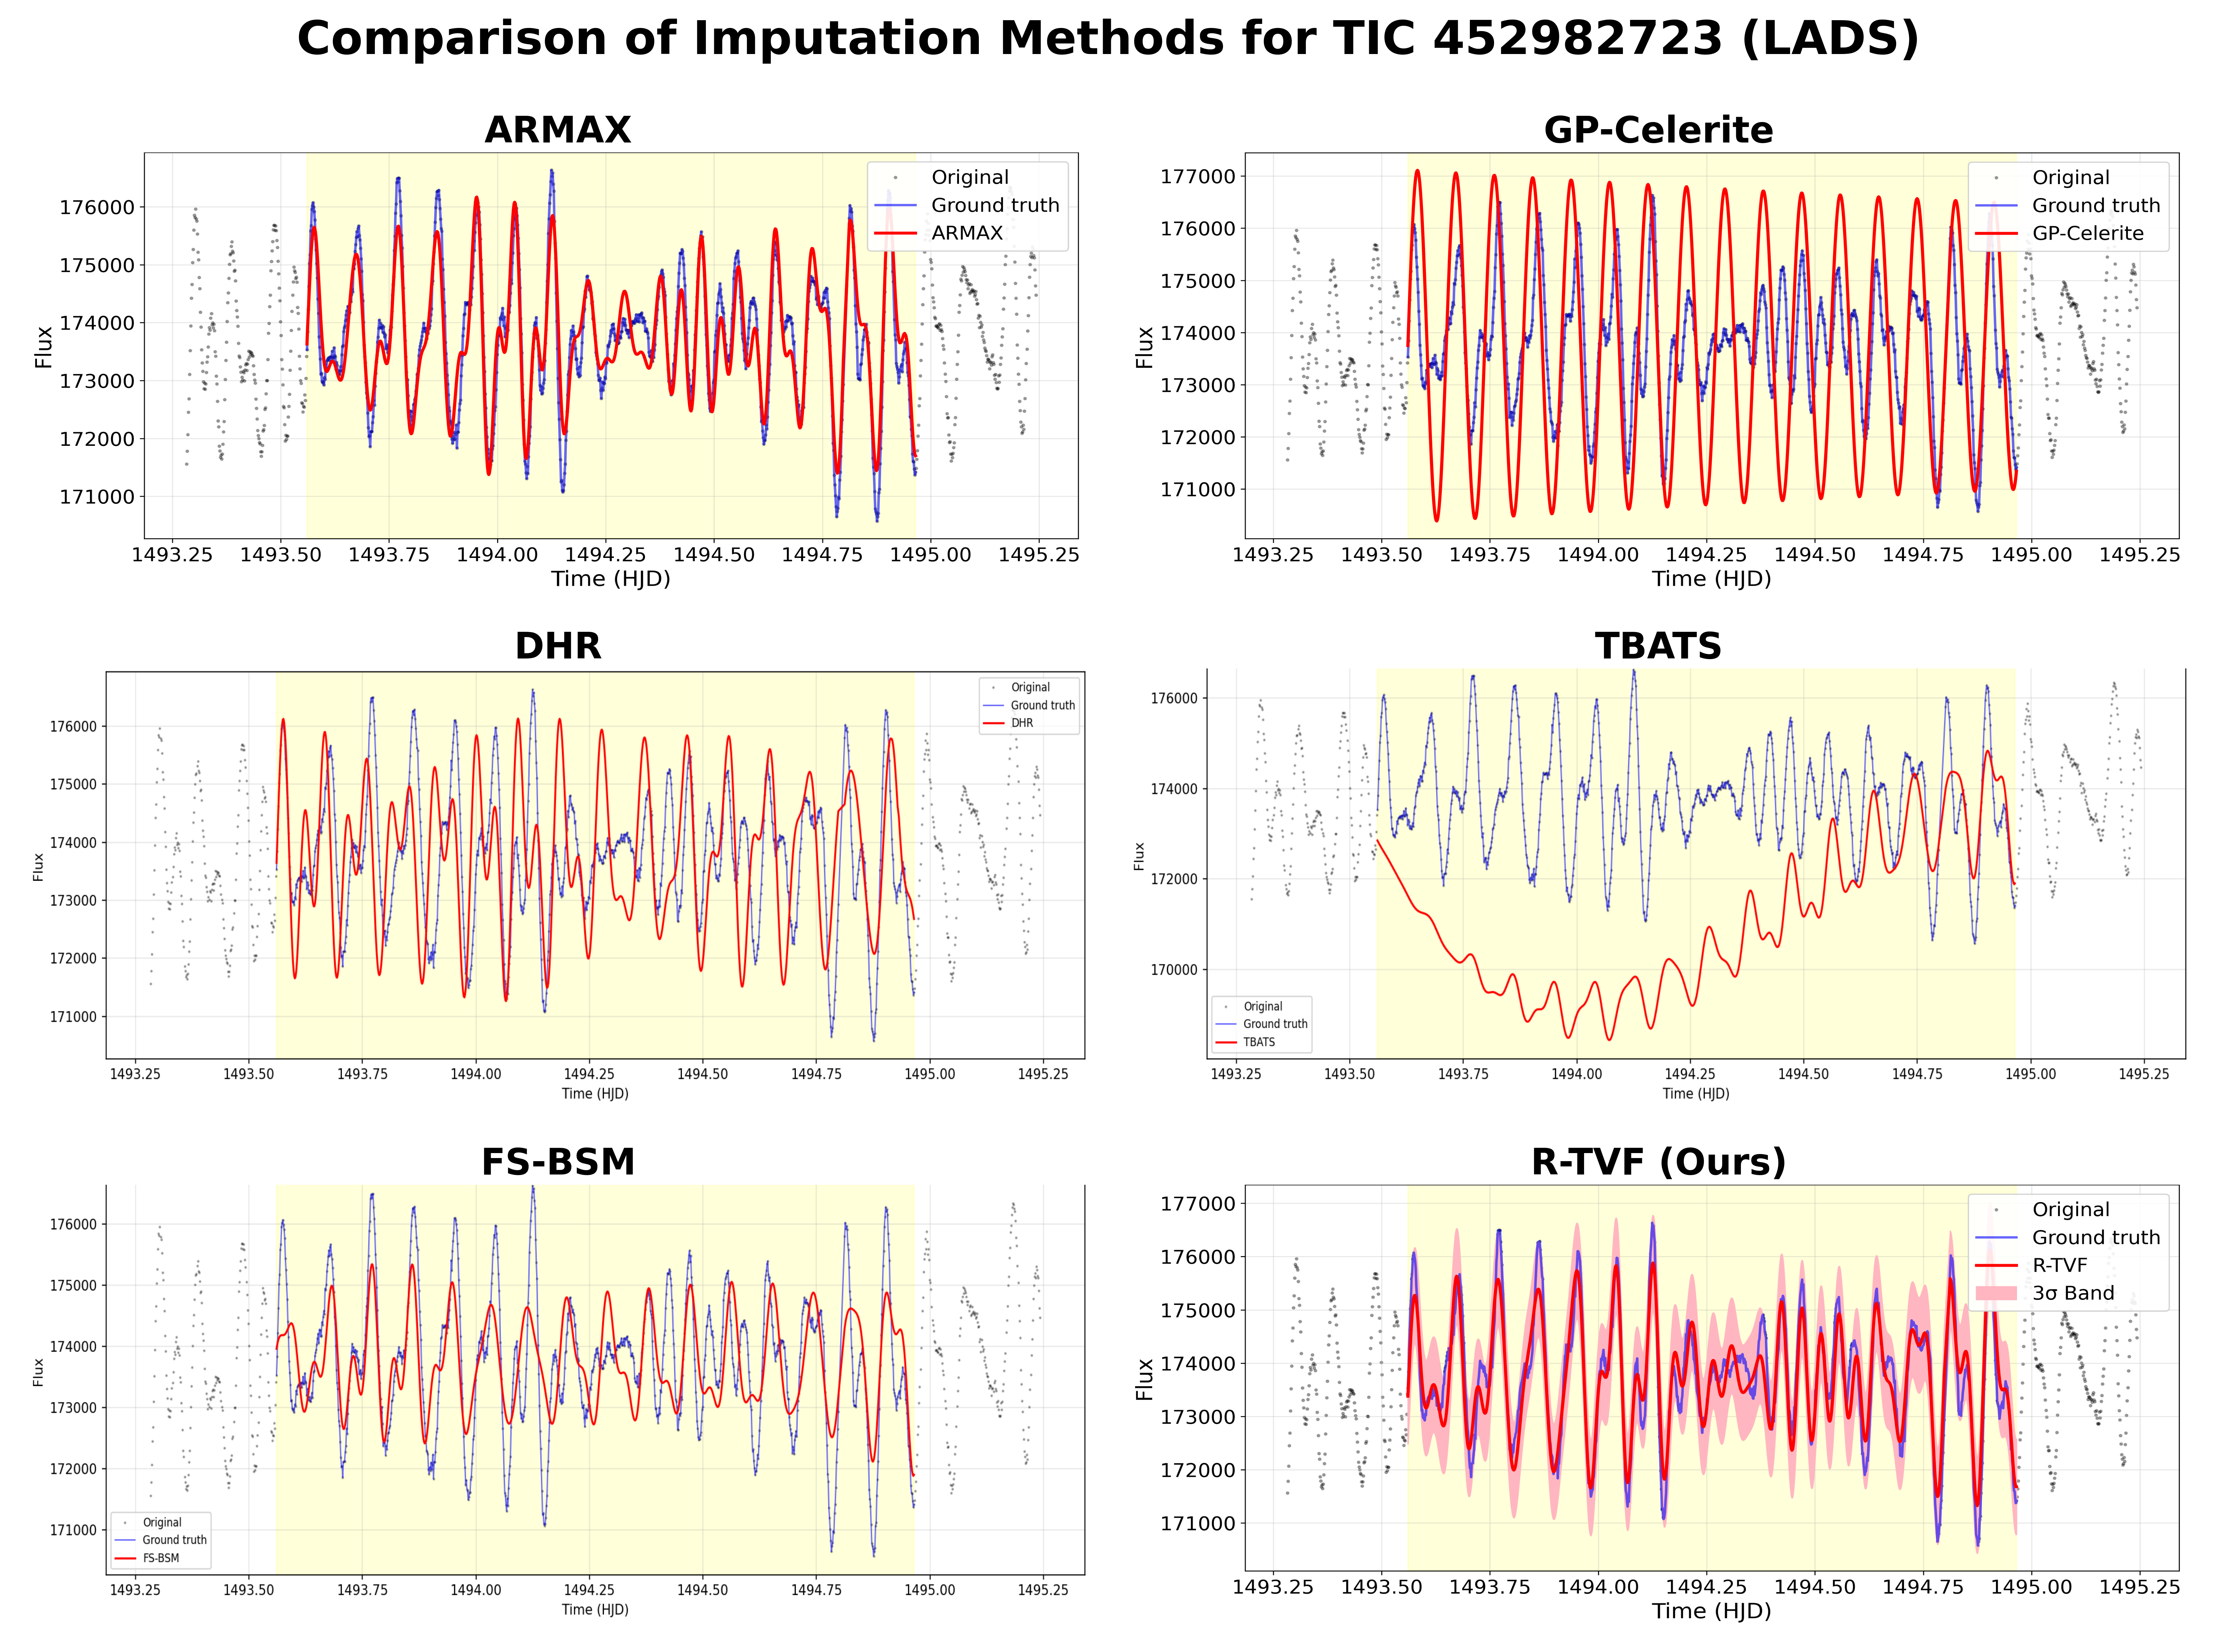
\includegraphics[width=0.9\linewidth]{Images/grid_comparison_TIC452982723_large.png}
  \caption{Comparison of imputation methods for the LADS star TIC 452982723. The $3\sigma$ analytical uncertainty band (shaded pink) bounds the R-TVF predictions.}
  \label{fig:grid_lads}
\end{figure}

\subsection{Evaluation for Gaps of $N=2000$}

The results of this analysis ($N=2000$), summarized in Tables \ref{tab:cv_hads_2000} and \ref{tab:cv_lads_2000}, confirm the superior performance of R-TVF, maintaining high accuracy for HADS stars ($R^2 = 0.968$) and outperforming all methods in the LADS stars ($R^2 = 0.761$). While ARMAX remained competitive, achieving the lowest MSE for HADS stars ($45.3 \times 10^6$), the performance of the alternative harmonic and state-space methods (DHR, FS-BSM, TBATS) decreased under these wider gaps, with FS-BSM dropping to $R^2 = 0.885$ (HADS) and $R^2 = 0.725$ (LADS), while DHR, TBATS, and GP-Celerite yielded lower accuracies. Figures \ref{fig:robustness_hads_grid} and \ref{fig:robustness_lads_grid} confirm this stability, showing that R-TVF maintains phase coherence and prevents signal degradation even across these bigger gaps.


\begin{table*}[htbp]
\centering
\caption{Cross-validation results for HADS stars ($N=2000$). The computational time is decomposed into Lomb-Scargle Periodogram estimation (LS) and final Model Fit (Fit).}
\label{tab:cv_hads_2000}
\resizebox{0.95\textwidth}{!}{%
\begin{tabular}{lcccccc}
\toprule
\textbf{Method} & \textbf{MAE} & \textbf{MSE ($\times 10^6$)} & \textbf{MAPE (\%)} & \textbf{$R^2$} & \textbf{Total Time (s)} & \textbf{LS / Fit (s)} \\
\midrule
ARMAX & 1997 $\pm$ 5217 & \textbf{45.3 $\pm$ 227.7} & 216.1 $\pm$ 139.5 & 0.891 $\pm$ 0.119 & 47.7 $\pm$ 29.1 & 0.05 / 47.65 \\
GP-Celerite & 11314 $\pm$ 45551 & 2746.3 $\pm$ 16195.9 & 717.7 $\pm$ 296.5 & -0.061 $\pm$ 0.356 & \textbf{0.71 $\pm$ 0.16} & 0.03 / 0.68 \\
DHR & 7510 $\pm$ 12145 & 215.2 $\pm$ 682.5 & 550.5 $\pm$ 285.3 & 0.185 $\pm$ 0.254 & 28.3 $\pm$ 6.2 & 0.05 / 28.25 \\
TBATS & 5150 $\pm$ 8500 & 132.6 $\pm$ 410.2 & 410.4 $\pm$ 220.5 & 0.448 $\pm$ 0.162 & 32.5 $\pm$ 8.1 & 0.04 / 32.46 \\
FS-BSM & 2050 $\pm$ 4800 & 68.5 $\pm$ 250.2 & 230.4 $\pm$ 140.5 & 0.885 $\pm$ 0.125 & 45.8 $\pm$ 12.5 & 0.05 / 45.75 \\
R-TVF (ours) & \textbf{1893 $\pm$ 7713} & 96.9 $\pm$ 559.1 & \textbf{98.6 $\pm$ 86.8} & \textbf{0.968 $\pm$ 0.051} & 9.2 $\pm$ 3.0 & 0.06 / 9.14 \\
\bottomrule
\end{tabular}%
}
\end{table*}




\begin{table*}[htbp]
\centering
\caption{Cross-validation results for LADS stars ($N=2000$). The computational time is further decomposed into Lomb-Scargle Periodogram estimation (LS) and final Model Fit (Fit).}
\label{tab:cv_lads_2000}
\resizebox{0.95\textwidth}{!}{%
\begin{tabular}{lcccccc}
\toprule
\textbf{Method} & \textbf{MAE} & \textbf{MSE ($\times 10^3$)} & \textbf{MAPE (\%)} & \textbf{$R^2$} & \textbf{Total Time (s)} & \textbf{LS / Fit (s)} \\
\midrule
ARMAX & 243 $\pm$ 451 & 384.6 $\pm$ 1710.3 & 21.0 $\pm$ 25.6 & 0.738 $\pm$ 0.173 & 72.6 $\pm$ 46.9 & 0.05 / 72.55 \\
GP-Celerite & 622 $\pm$ 1032 & 2125.1 $\pm$ 5941.5 & 62.5 $\pm$ 90.3 & -0.163 $\pm$ 0.391 & \textbf{0.73 $\pm$ 0.16} & 0.02 / 0.71 \\
DHR & 510 $\pm$ 850 & 1450.4 $\pm$ 4450.2 & 48.4 $\pm$ 45.1 & 0.098 $\pm$ 0.380 & 31.4 $\pm$ 7.2 & 0.04 / 31.36 \\
TBATS & 485 $\pm$ 660 & 1285.6 $\pm$ 3480.5 & 45.2 $\pm$ 35.4 & 0.145 $\pm$ 0.210 & 35.1 $\pm$ 9.3 & 0.05 / 35.05 \\
FS-BSM & 265 $\pm$ 420 & 410.5 $\pm$ 1850.2 & 25.0 $\pm$ 22.5 & 0.725 $\pm$ 0.180 & 48.2 $\pm$ 14.1 & 0.06 / 48.14 \\
R-TVF (ours) & \textbf{217 $\pm$ 380} & \textbf{287.6 $\pm$ 1192.2} & \textbf{16.8 $\pm$ 13.4} & \textbf{0.761 $\pm$ 0.161} & 9.8 $\pm$ 3.3 & 0.06 / 9.72 \\
\bottomrule
\end{tabular}%
}
\end{table*}


    
\begin{figure}[pos=htbp]
  \centering
  \includegraphics[width=1\linewidth]{Images/rtvf_grid_hads_large.png}
  \caption{Analysis sample of 16 HADS stars with extended gaps ($N=2000$). Red lines represent the R-TVF imputation, and blue lines indicate the ground truth. The $3\sigma$ analytical uncertainty band (shaded pink) bounds the R-TVF predictions.}
  \label{fig:robustness_hads_grid}
\end{figure}

\begin{figure}[pos=htbp]
  \centering
  \includegraphics[width=1\linewidth]{Images/rtvf_grid_lads_large.png}
  \caption{Analysis sample of 16 LADS stars with extended gaps ($N=2000$). Red lines represent the R-TVF imputation, and blue lines indicate the ground truth. The $3\sigma$ analytical uncertainty band (shaded pink) bounds the R-TVF predictions.}
  \label{fig:robustness_lads_grid}
\end{figure}



{\color{blue}
\subsection{Frequency-Domain Validation} \label{sec:frequency_validation}

To compare the dominant frequencies and amplitudes of the original and reconstructed light curves, we computed the Lomb-Scargle periodogram for four representative stars: two HADS (HD~146953, VZ~Cnc) and two LADS (TIC~242944780, TIC~452982723). Following our experimental set-up, we removed a gap of $N=1000$ points from each light curve and analyzed three scenarios: the original complete light curve (ground truth), the series without imputation (unimputed), and the signal reconstructed with R-TVF. This comparison allows us to evaluate whether imputing the missing data with R-TVF provides a more accurate spectrum than leaving the gap unimputed.


%@maria, aquí está lo que me dijiste que explicara en la llamada.
Figure~\ref{fig:freq_grid_2x2} shows the frequency domain of the ground truth (black), the unimputed gapped series (orange), and the R-TVF reconstruction (red). The plot appears primarily red because the R-TVF spectrum lies directly on top of the black ground-truth spectrum across the entire frequency range, confirming that R-TVF recovers the full set of oscillation frequencies and their corresponding amplitudes. While the unimputed series also captures the dominant frequencies such as $f_1$, it generates multiple spurious peaks across the spectrum that do not correspond to true stellar oscillation frequencies.
}

%In contrast, R-TVF suppresses these artificial peaks and faithfully preserves the true frequency spectrum of the light curve. %lo comento porque es redundante y no me cuadra bien aquí.

\begin{figure}[pos=htbp]
  \centering
  \includegraphics[width=0.97\linewidth]{Images/grid_2x2_frequency_spectrum.png}
  \caption{{\color{blue}Frequency domain of the ground truth (black), unimputed gapped series (orange), and R-TVF reconstruction (red) for two HADS (HD~146953, VZ~Cnc) and two LADS (TIC~242944780, TIC~452982723) stars. The red R-TVF spectrum overlaps the black ground-truth spectrum across all frequencies, while the visible orange peaks represent spurious artifacts introduced by the missing-data gap. The dominant frequency $f_1$ is marked with a dashed line.}}
  \label{fig:freq_grid_2x2}
\end{figure}




\subsection{Sensitivity Analysis}

We conducted a sensitivity analysis of the three hyperparameters of R-TVF: the number of harmonic components ($K$), the polynomial degree ($d$) controlling time-varying amplitude, and the regularization strength ($\lambda$) for gaps of $N=1000$. Figures~\ref{fig:sensitivity_lambda00} to \ref{fig:sensitivity_lambda010} show the median $R^2$ performance for HADS and LADS stars across different hyperparameter settings.


\begin{figure}[pos=htbp]
  \centering

  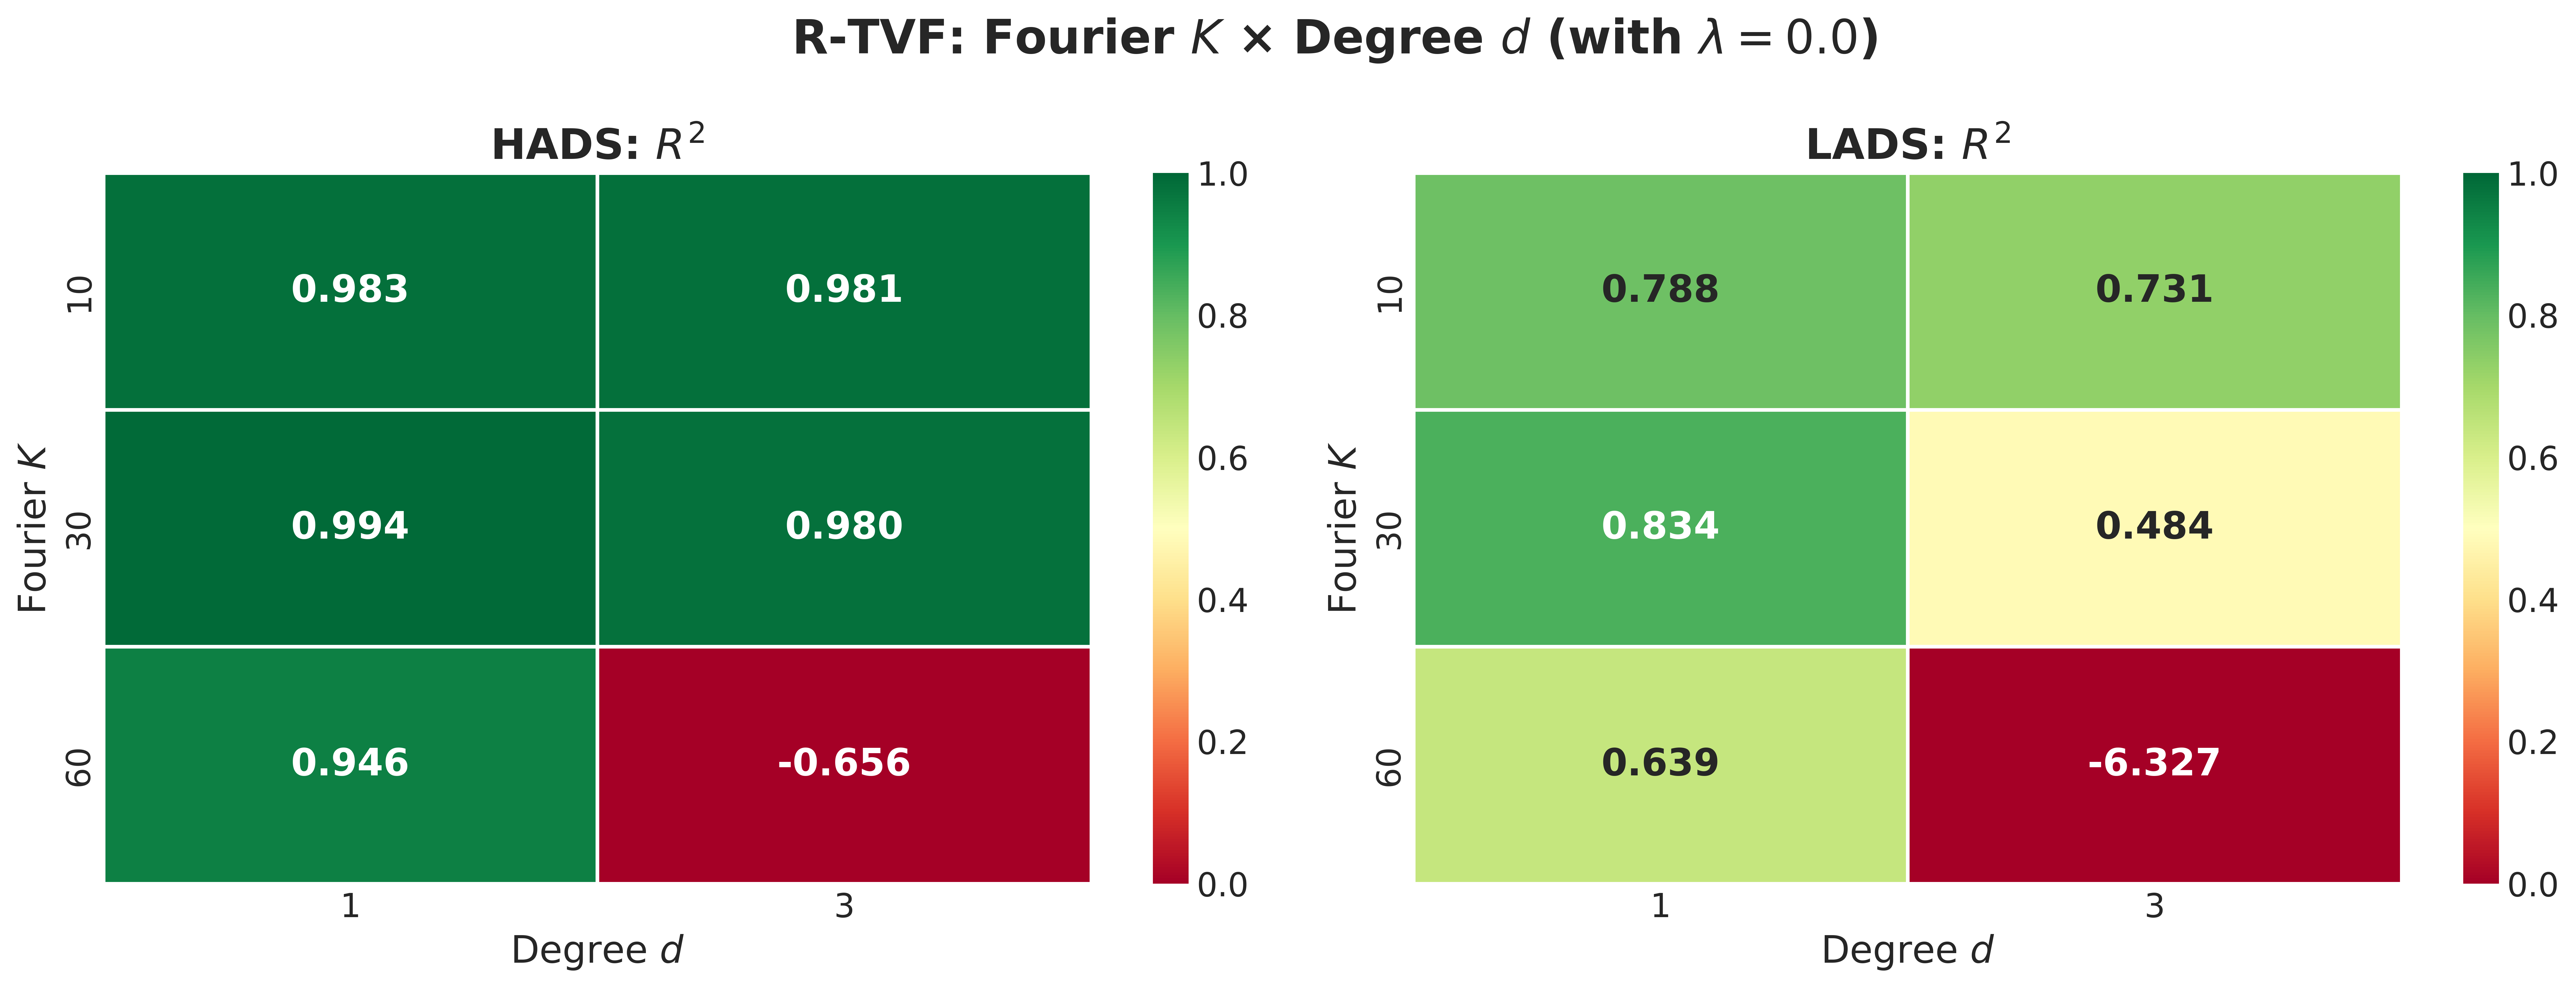
\includegraphics[width=0.621\linewidth]{Images/heatmap_K_vs_degree_lambda0_0_median.png}
  \caption{R-TVF sensitivity to $K$ and $d$ with $\lambda = 0.0$ (No regularization).}
  \label{fig:sensitivity_lambda00}

  %\vspace{0.4cm} % Separación entre imágenes

  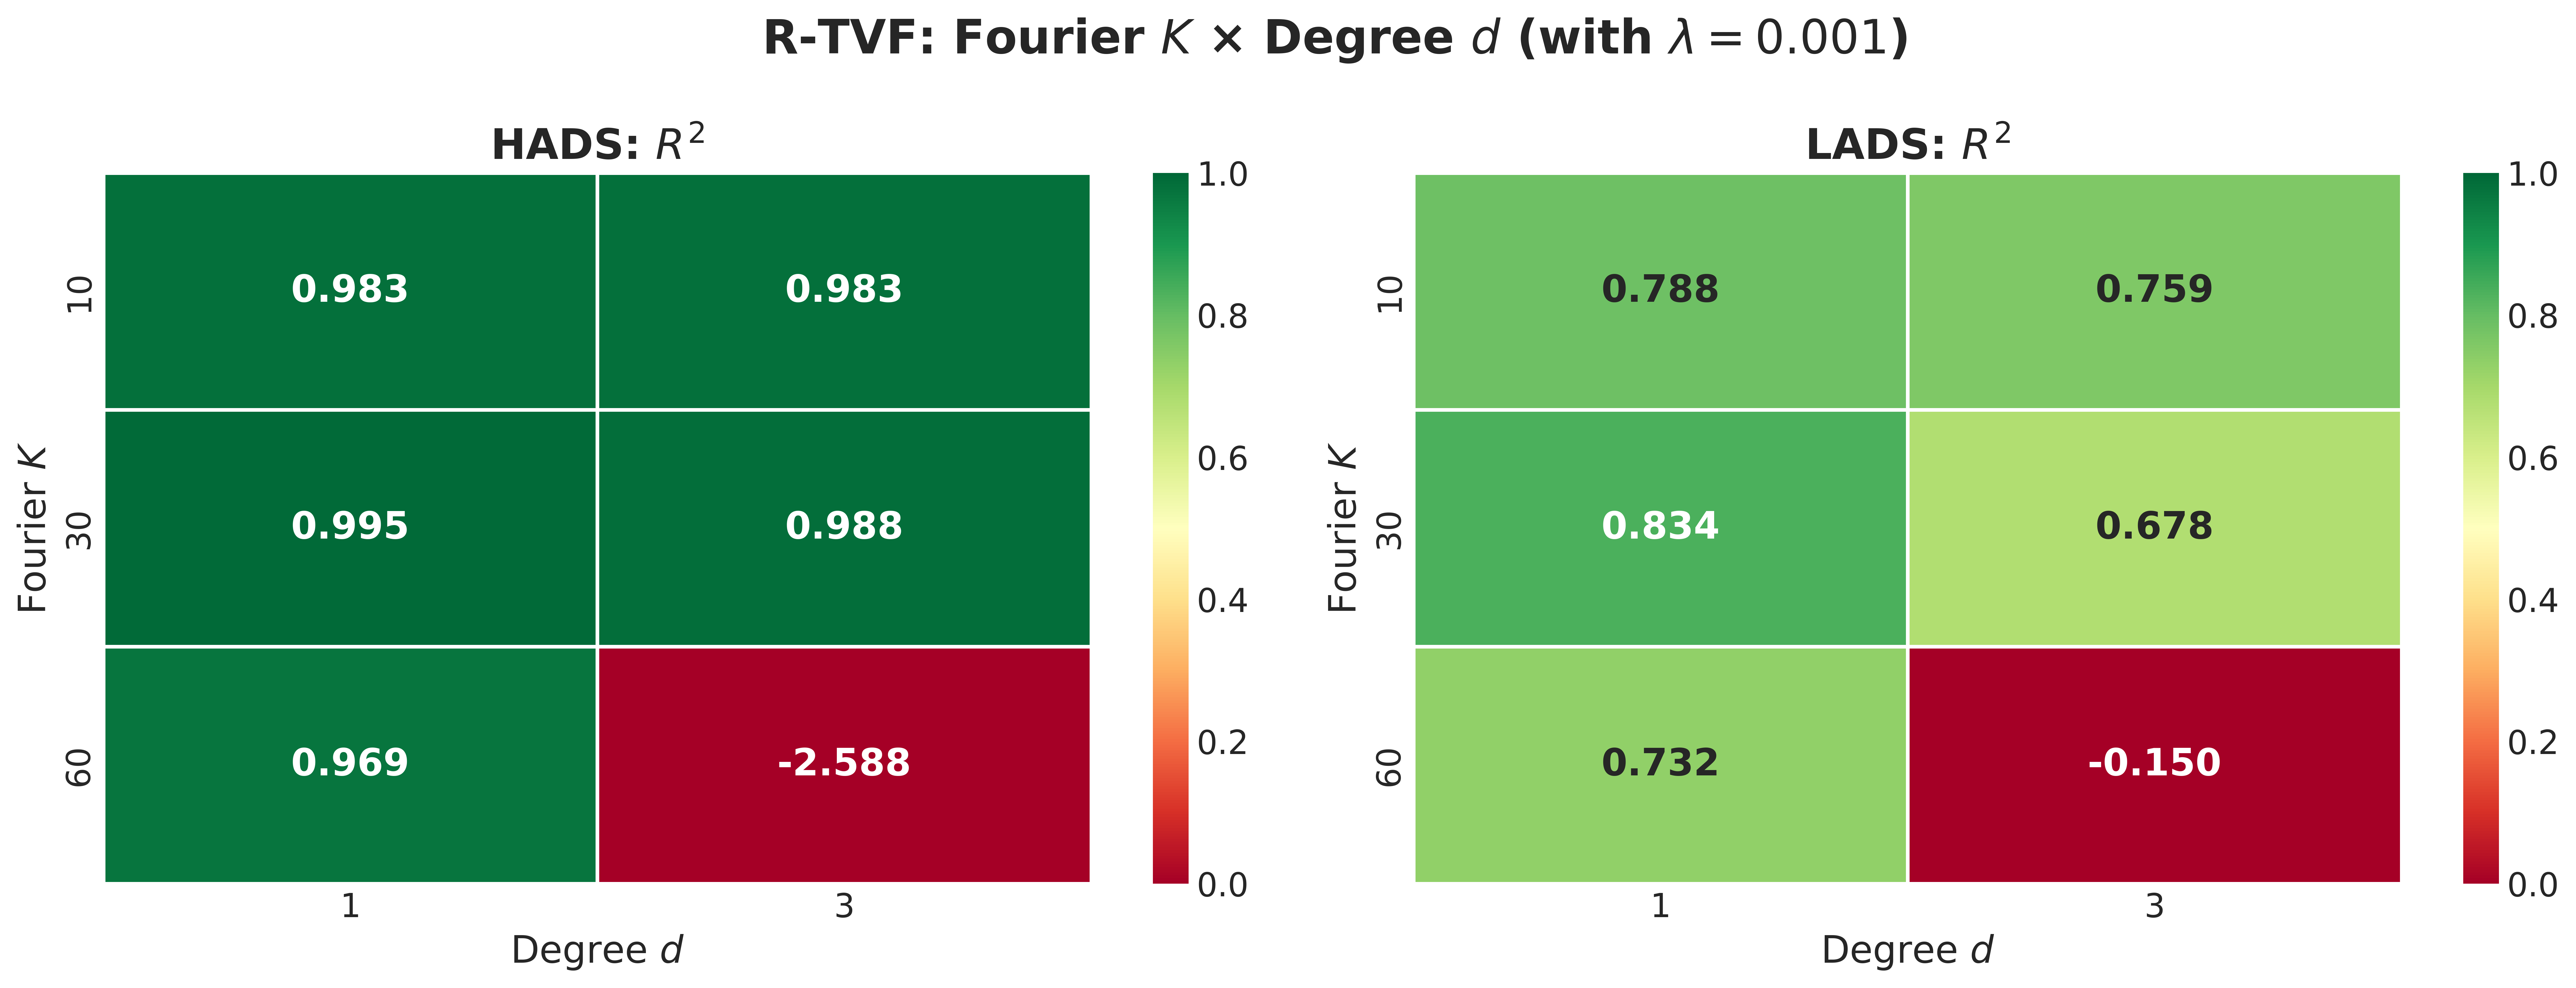
\includegraphics[width=0.621\linewidth]{Images/heatmap_K_vs_degree_lambda0_001_median.png}
  \caption{R-TVF sensitivity to $K$ and $d$ with $\lambda = 0.001$ (Weak regularization).}
  \label{fig:sensitivity_lambda001}

  %\vspace{0.4cm}

  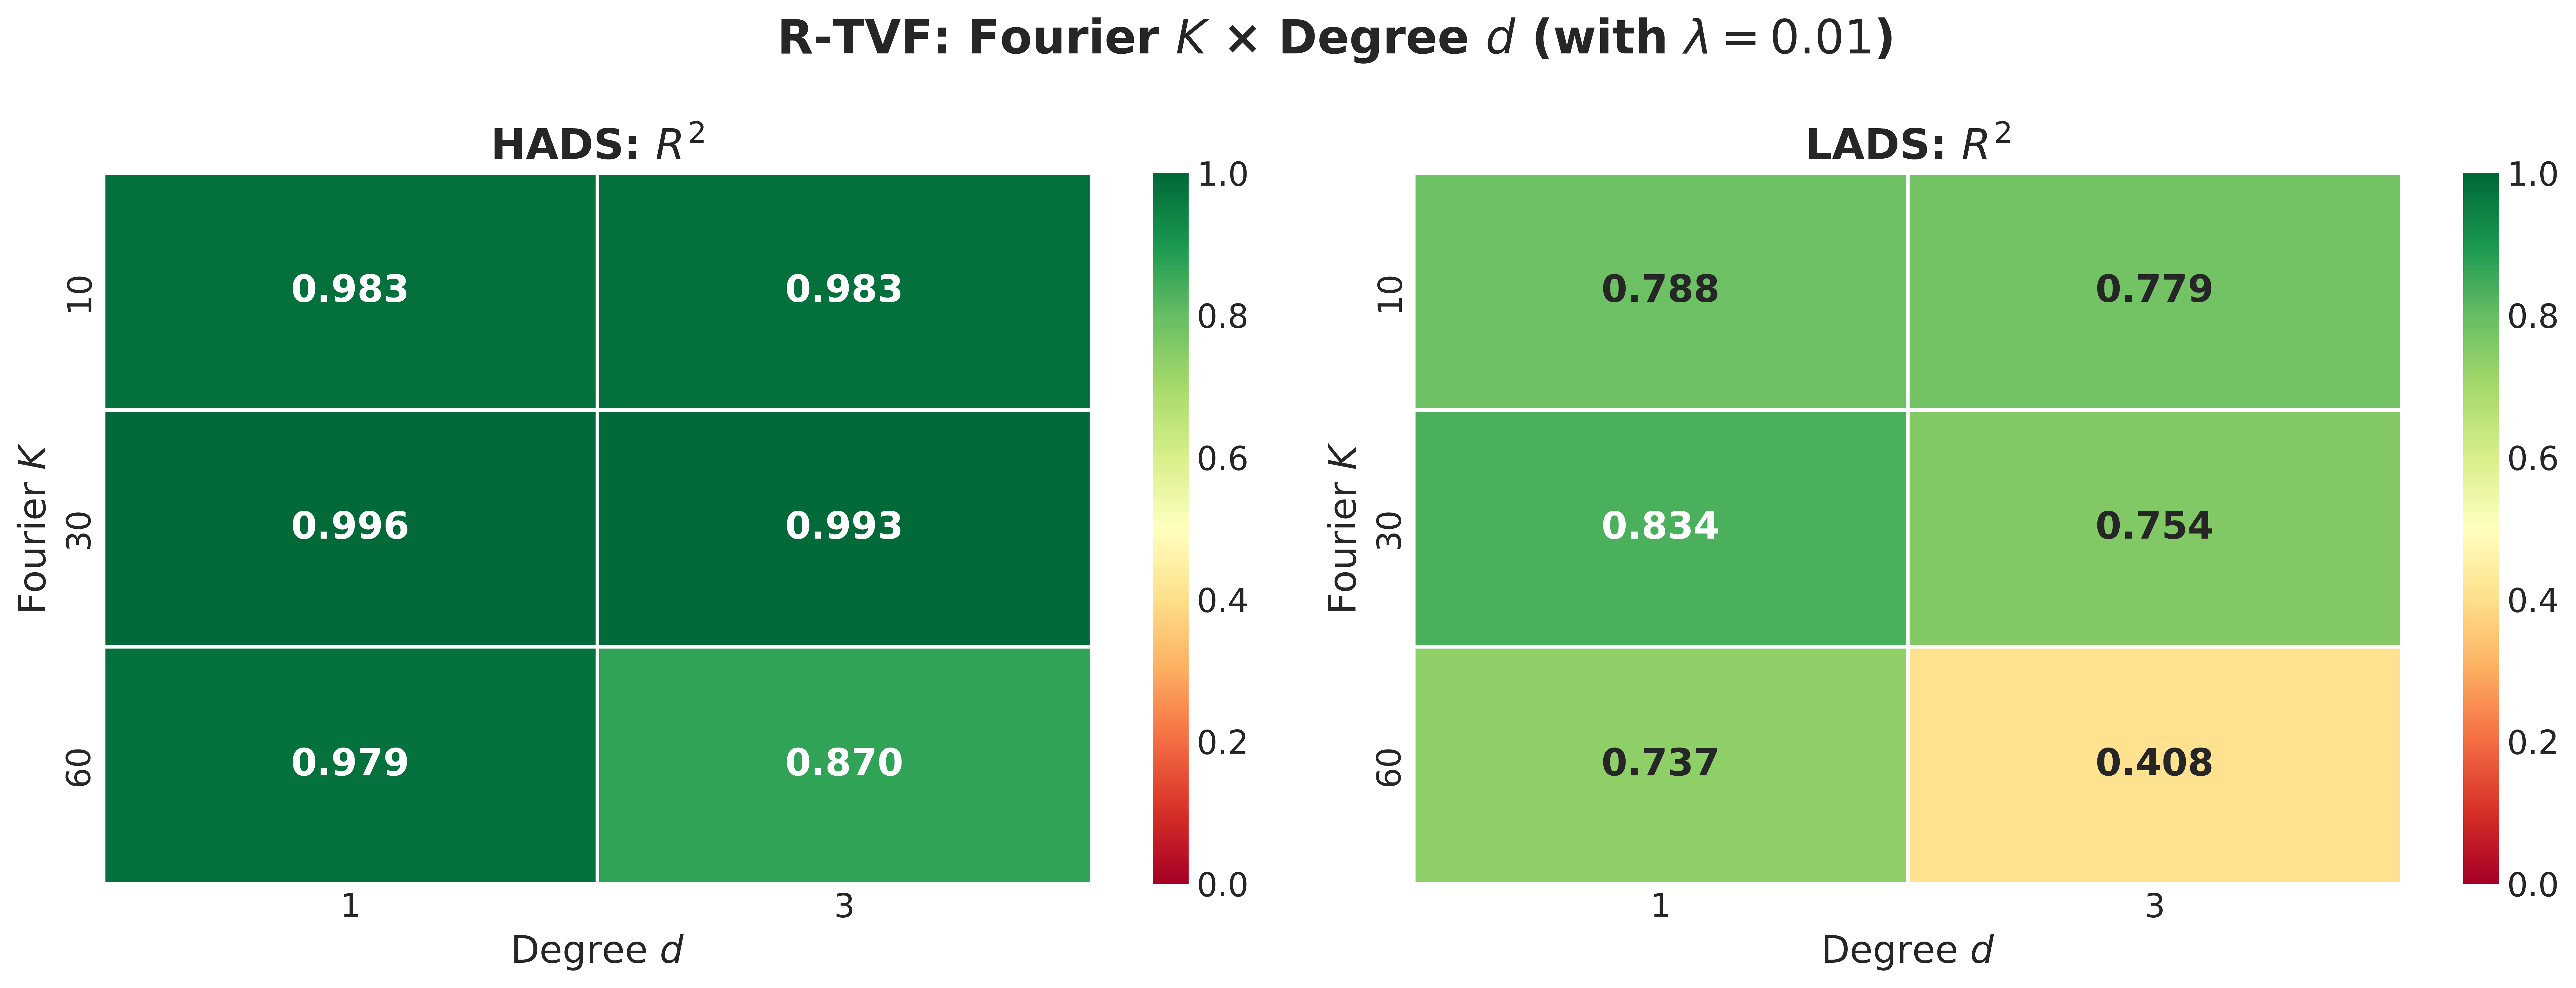
\includegraphics[width=0.621\linewidth]{Images/heatmap_K_vs_degree_lambda0_01_median.png}
  \caption{R-TVF sensitivity to $K$ and $d$ with $\lambda = 0.01$ (Moderate regularization).}
  \label{fig:sensitivity_lambda01}

  %\vspace{0.4cm}

  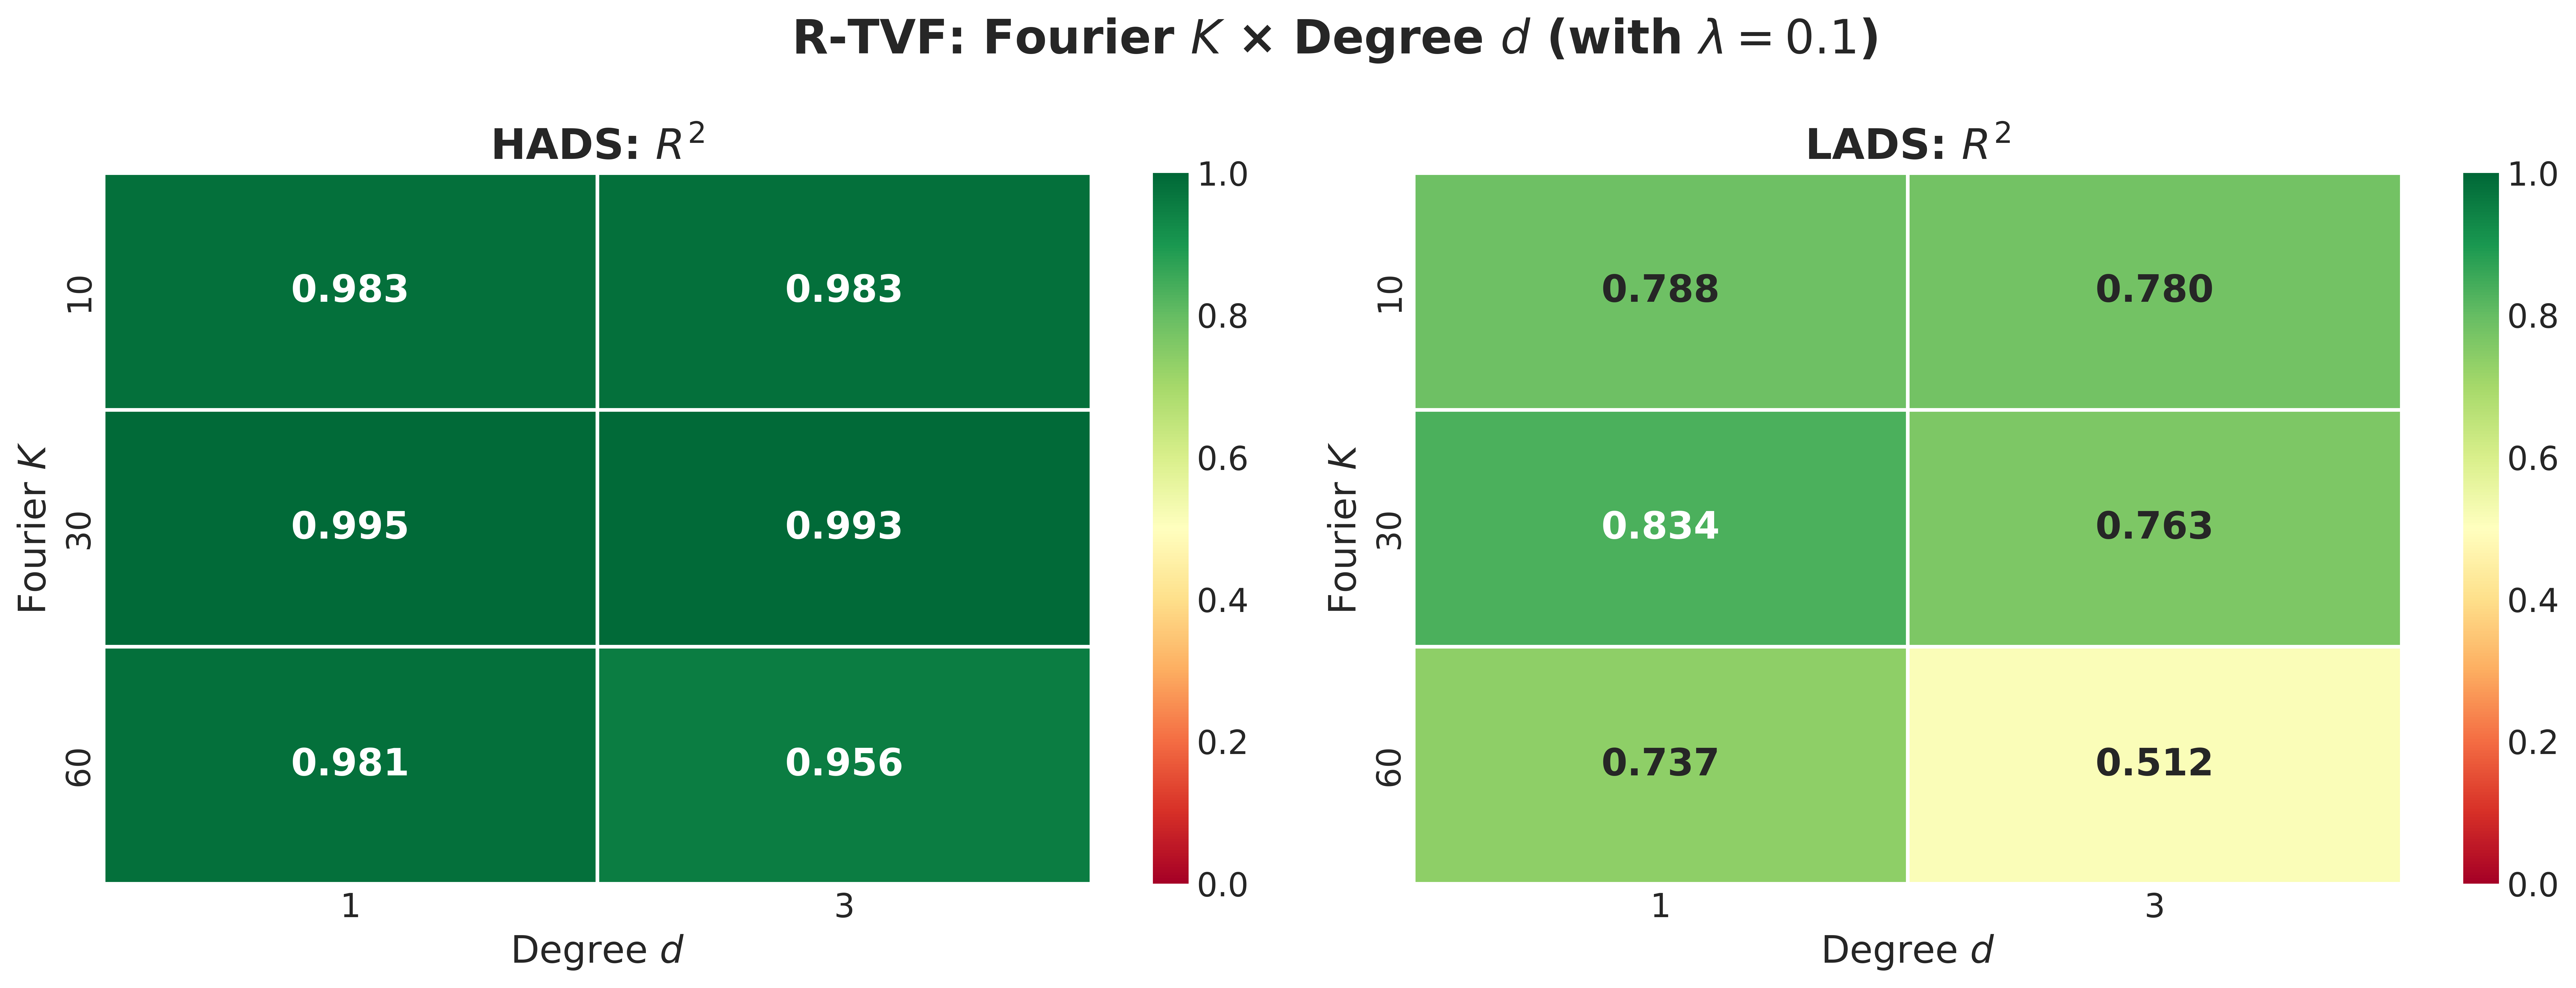
\includegraphics[width=0.621\linewidth]{Images/heatmap_K_vs_degree_lambda0_1_median.png}
  \caption{R-TVF sensitivity to $K$ and $d$ with $\lambda = 0.1$ (Strong regularization).}
  \label{fig:sensitivity_lambda010}
\end{figure}


Results without or with weak regularization ($\lambda=0.0$ in Fig. \ref{fig:sensitivity_lambda00} and $\lambda=0.001$ in Fig. \ref{fig:sensitivity_lambda001}) reveal a performance degradation as model complexity increases. While simple configurations ($d=1$) remain robust, increasing the polynomial degree to $d=3$ combined with a high harmonic density ($K=60$) causes a severe drop in performance. This degradation is particularly pronounced in LADS stars.

Regarding regularization, moderate values ($\lambda=0.01$, Fig. \ref{fig:sensitivity_lambda01}) mitigate the negative scores, but the strongest configuration tested ($\lambda=0.1$, Fig. \ref{fig:sensitivity_lambda010}) yields the most robust performance. Specifically, LADS stars with $d=3$ and $K=30$ improve from a median $R^2=0.754$ to $R^2=0.763$, while maintaining the peak median accuracy in the optimal linear cases ($R^2 \approx 0.834$, whereas Table~\ref{tab:cv_lads} reports the mean $R^2$ of $0.816$).



\subsection{Statistical Significance Analysis}

To assess the statistical reliability of the results, we conducted a non-parametric statistical analysis \cite{demvsar2006statistical}. Specifically, we applied the Friedman test to detect global differences among the methods, followed by the Wilcoxon signed-rank test with Holm-Bonferroni correction for pairwise comparisons. To satisfy the independence assumption of the statistical tests, we aggregated the cross-validation results by star first, averaging the metrics across the 5 folds for each of the 72 stars before applying the tests \cite{demvsar2006statistical}.

The Friedman test operates under the null hypothesis that all algorithms perform equivalently. As shown in Table \ref{tab:friedman_combined}, the test was conducted on 72 independent stars. The resulting test statistics ($\chi^2 = 294.83$ for $N=1000$ and $\chi^2 = 322.09$ for $N=2000$) yield $p$-values close to zero ($p < 0.001$), rejecting the null hypothesis. The table also reports the average rankings, where R-TVF achieves the lowest (best) mean ranks of $1.24$ and $1.39$, confirming its consistent superiority across the dataset. ARMAX ranks second, while the other harmonic methods perform worse.


\begin{table}[htbp]
\centering
\caption{Friedman test results and average rankings comparing methods at the star level ($N=72$ independent stars). The rankings are based on $R^2$ performance (lower rank corresponds to better performance).}
\label{tab:friedman_combined}
\begin{tabular}{lcc}
\toprule
\textbf{Statistic / Method} & \textbf{Value ($N=1000$)} & \textbf{Value ($N=2000$)} \\
\midrule
\multicolumn{3}{c}{\textit{Friedman Statistic}} \\
 Evaluations (Stars) & 72 & 72 \\
Chi-square ($\chi^2$) & 294.83 & 322.09 \\
$p$-value & $<$ 0.001 & $<$ 0.001 \\
\midrule
\multicolumn{3}{c}{\textit{Average Ranks (Lower is Better)}} \\
\textbf{R-TVF (ours)} & \textbf{1.24} & \textbf{1.39} \\
ARMAX & 2.29 & 2.08 \\
FS-BSM & 2.58 & 2.61 \\
TBATS & 4.43 & 4.04 \\
DHR & 5.06 & 4.89 \\
GP-Celerite & 5.40 & 5.99 \\
\bottomrule
\end{tabular}
\end{table}




Table \ref{tab:nemenyi_combined} summarizes the pairwise Wilcoxon signed-rank post-hoc comparisons between R-TVF and each method across both gap size scenarios, with Holm-Bonferroni correction. Following current recommendations for robust statistical significance \cite{lakens2018justify}, we adopt a threshold of $p < 0.05$. The analysis confirms that R-TVF's performance advantage is statistically significant against all methods in both scenarios. Specifically, all pairwise comparisons yield $p < 0.001$ in the $N=1000$ scenario, while for $N=2000$, we obtain $p < 0.001$ against GP-Celerite, DHR, TBATS, and FS-BSM, and $p = 0.008$ against ARMAX.


\begin{table}[htbp]
\centering
\caption{Pairwise Wilcoxon signed-rank test results comparing R-TVF against baseline methods at the star level ($72$ stars) for both gap size scenarios. The table reports raw $p$-values and corrected $p$-values after Holm-Bonferroni correction. Corrected $p$-values $< 0.05$ indicate statistically significant differences.}
\label{tab:nemenyi_combined}
\resizebox{0.75\textwidth}{!}{%
\begin{tabular}{lccccc}
\toprule
 & \multicolumn{2}{c}{\textbf{Scenario $N=1000$}} & & \multicolumn{2}{c}{\textbf{Scenario $N=2000$}} \\
\cline{2-3} \cline{5-6}
\textbf{Comparison (R-TVF vs.)} & \textbf{Raw $p$-value} & \textbf{Corrected $p$-value} & & \textbf{Raw $p$-value} & \textbf{Corrected $p$-value} \\
\midrule
ARMAX & $<$ 0.001 & $<$ 0.001 & & 0.008 & 0.008 \\
GP-Celerite & $<$ 0.001 & $<$ 0.001 & & $<$ 0.001 & $<$ 0.001 \\
DHR & $<$ 0.001 & $<$ 0.001 & & $<$ 0.001 & $<$ 0.001 \\
TBATS & $<$ 0.001 & $<$ 0.001 & & $<$ 0.001 & $<$ 0.001 \\
FS-BSM & $<$ 0.001 & $<$ 0.001 & & $<$ 0.001 & $<$ 0.001 \\
\bottomrule
\end{tabular}%
}
\end{table}





\subsection{Discussion} \label{sec:discussion}

The superior performance of R-TVF across both scenarios ($N=1000$ and $N=2000$) can be understood by how each method fits the signal across the gap. Since all methods use the same dominant frequencies from the Lomb-Scargle periodogram, the differences arise from their fitting strategy. DHR, FS-BSM, and TBATS estimate the signal sequentially, propagating their parameters forward through the gap without data corrections; over large gaps, this leads to significant degradation. DHR and FS-BSM exhibit phase drift, with oscillations that progressively lose phase coherence with the true signal. TBATS fails to reproduce the oscillations of the true signal, resulting in waves with incorrect shapes and amplitudes. GP-Celerite tends to produce rigid, overly regular oscillations that do not adapt to the star's true amplitude modulation. In contrast, ARMAX relies on a global fit using all observed data (via numerical maximum likelihood estimation), unlike R-TVF's closed-form ridge solution, but both avoid the sequential propagation of parameters used by state-space methods, preserving phase coherence across the gap. However, ARMAX assumes constant amplitudes, limiting its accuracy for LADS stars where the oscillation amplitude varies over time. R-TVF overcomes this limitation by generalizing the static Fourier model with time-varying polynomial coefficients, allowing it to follow the amplitude modulation of LADS stars, resulting, for these stars, in a reduction of imputation error (MSE) by up to 25\% and execution time by over 80\% compared to ARMAX. While ARMAX achieves a lower mean MSE for HADS stars due to their high and constant amplitudes, R-TVF offers superior overall reconstruction quality (as measured by the mean $R^2$ coefficient) across both stellar families. {\color{blue}In this regard, while ARMAX provides an external comparison with static amplitudes, the direct structural ablation within R-TVF corresponds to setting the polynomial degree to $d=0$ (constant Fourier coefficients fitted via ridge regression). In both cases, keeping the Fourier coefficients constant limits the model's ability to follow the dynamic amplitude modulations of LADS stars.}%Furthermore, the direct structural ablation of R-TVF corresponds to setting the polynomial degree to $d=0$ (constant Fourier coefficients fitted via closed-form ridge regression), %demonstrating that the time-varying polynomial expansion ($d=1$) is required to capture amplitude modulations in LADS stars.}

{\color{blue}Regarding the frequency-domain validation, leaving the data unimputed introduces spurious peaks that can be easily misinterpreted as real stellar frequencies. By reconstructing the missing interval with R-TVF, we suppress these false peaks and recover both the dominant frequencies and amplitudes of the original signal. This confirms that R-TVF preserves the frequency information of the light curves, which is necessary for asteroseismic analysis.}

Regarding the sensitivity analysis, the polynomial degree shows that although a cubic degree ($d=3$) increases the flexibility of the time-varying amplitude evolution, it increases the risk of the Runge phenomenon within the unobserved gap, as indicated by low or negative $R^2$ values. Second, the number of Fourier components $K=30$ proves optimal because it captures dominant oscillation modes without overfitting. Finally, the regularization parameter $\lambda$ acts as a stabilizer for the polynomial expansion: we found that strong regularization ($\lambda=0.1$) prevents the polynomial coefficients from diverging in the unobserved region while preserving the smooth evolution of the flux amplitude. By evaluating the model at $\lambda=0$, we perform an ablation study of the regularization penalty, confirming its necessity to prevent overfitting. Consequently, the analysis confirms that a linear degree ($d=1$), combined with $K=30$ and $\lambda=0.1$, captures the general variability of all HADS and LADS stars. Therefore, we propose this configuration as it maximizes performance, recovering the dominant frequencies needed for asteroseismic analysis.

{\color{blue}Finally, regarding the scope of the experimental design, our evaluation focuses exclusively on a single continuous missing-data gap of length $N=1000$ and $N=2000$, which simulates extended telemetry downlink windows. While we designed the R-TVF method to bridge such wide continuous missing-data gaps, this performance does not automatically extend to other missing-data patterns. Highly fragmented observations, short intermittent missing-data gaps, or multi-gap distributions present distinct spectral window functions and phase-tracking challenges.}



\section{Conclusion} \label{sec:conclusion}

This study introduces R-TVF, a frequency-informed imputation method designed to reconstruct missing data in photometric time series. By leveraging the intrinsic oscillation properties of stars, R-TVF addresses the limitations of general-purpose imputation techniques. Our empirical validation is specifically focused on 72 Delta Scuti stars observed by the TESS mission. Our analysis on these stars demonstrates that R-TVF outperforms static Fourier models and sequentially fitted harmonic methods.  Specifically, R-TVF achieves a mean $R^2$ between 0.968 and 0.987 for HADS stars, and between 0.761 and 0.816 for LADS stars, representing an accuracy improvement of 3\% to 9\% over the second-best method (ARMAX), while reducing execution time by 80\% to 88\% across all analyzed gap sizes. The statistical analysis confirms the significance of these results, validating that a closed-form fit with time-varying polynomial coefficients outperforms these methods, particularly for large data gaps. R-TVF effectively models the dynamic evolution of oscillation amplitudes through a regularized polynomial expansion, preventing overfitting. Because the current empirical scope is constrained to the Delta Scuti family, TESS data, {\color{blue}and single contiguous gaps}, in the future we intend to extend this validation to other stars, different missions, {\color{blue}and diverse missing-data patterns (such as intermittent and multi-gap patterns)} to achieve broader generalization.

%referencias al final.
%\newpage 

\section*{CRediT authorship contribution statement}
\textbf{Alberto Durán-López:} Validation, Investigation, Writing- Original Draft. \textbf{Daniel Bolaños-Martinez:} Investigation, Writing- Review \& Editing. \textbf{Zakaria Sahraoui El Ouahabi:} Validation, Investigation, Writing- Review \& Editing. \textbf{Antonio García Hernández:} Methodology, Validation, Resources, Investigation, Writing- Review \& Editing, Supervision, Project administration. \textbf{Juan Carlos Suárez:} Methodology, Validation, Resources, Investigation, Writing- Review \& Editing, Supervision. \textbf{Maria Bermudez-Edo:} Investigation, Writing- Review \& Editing, Supervision, Project administration.

\section*{Data availability}
Data will be made available on request.

\section*{Declaration of competing interest}
The authors declare that they have no known competing financial interests or personal relationships that could have appeared to influence the work reported in this paper.

\section*{Acknowledgements}

This work was supported by projects PID2023-149185OB-I00 and PID2023-149439NB-C43 funded by MICIU/AEI/10.13039/501100011033 and ERDF/EU; and by Grant C-SEJ-128-UGR23 funded by the Consejería de Universidad, Investigación e Innovación of the Junta de Andalucía and by the ERDF, EU.

%\appendix
%\section{My Appendix}
%Appendix sections are coded under \verb+\appendix+.

%\printcredits

%% Loading bibliography style file
%\bibliographystyle{model1-num-names}
%\bibliographystyle{cas-model2-names}
\bibliographystyle{elsarticle-num}

% Loading bibliography database
\bibliography{cas-refs}

\end{document}

